\documentclass[12pt, a4paper]{article} % свойства докуменат
\usepackage[utf8]{inputenc} % хотим нормальную кодировку
\usepackage[T2A]{fontenc} % тип шрифта, по-моему
\usepackage[russian]{babel} % русские буквы и обозначения
\usepackage{graphicx, xcolor} % графика
\usepackage{subfiles} % царская разбивка на много файлов
\usepackage{amsmath} % различные нужные символы, типа \geqslant
\usepackage{amssymb} % еще немного символов
\usepackage{import} % для включения рисунков
\usepackage{xifthen}
\usepackage{pdfpages}
\usepackage{transparent}
\usepackage{titlesec} % для настройки заголовков и секций вообще
\usepackage{caption} % для подписей к рисункам на 2 строки
\usepackage[outdir=./figures/]{epstopdf}
\usepackage{multicol}
\usepackage{float}
\usepackage{mathrsfs}

% комманда для царского добавления в документ векторной графики
\newcommand{\incfig}[1]{%
    \def\svgwidth{\columnwidth}
    \import{figures/}{#1.pdf_tex}
}
\pdfsuppresswarningpagegroup=1

\newcommand\eqdef{\stackrel{\text{\tiny def}}{=}}

\newtheorem{Th}{Теорема}

% русские знаки нестрогих неравенств
\renewcommand{\le}{\leqslant}
\renewcommand{\ge}{\geqslant}
\renewcommand{\emptyset}{\varnothing}
\renewcommand{\phi}{\varphi}
\renewcommand{\epsilon}{\varepsilon}

\newcommand{\Real}{\mathbb{R}}
\newcommand{\inner}[2]{\bigl< #1, #2 \bigr>}

\newcommand*{\hm}[1]{#1\nobreak\discretionary{}%
            {\hbox{\mathsurround=0pt #1}}{}}

\titleformat{\section}{\normalfont\Large\bfseries}{\thesection.}{1em}{}
\titleformat{\subsection}{\normalfont\Large\bfseries}{\thesubsection.}{1em}{}

\DeclareMathOperator{\conv}{conv}
\DeclareMathOperator*{\argmax}{argmax}
\DeclareMathOperator*{\Argmax}{Argmax}
\DeclareMathOperator{\sgn}{sgn}

% \counterwithin{section}{part}

\graphicspath{~/sa/oc_prac/lab_1/report/figures}

\begin{document}

\subfile{titul.tex}

\tableofcontents

\newpage

\part{Теоретическая часть}

\section{Постановка задач}

Движение ракеты в вертикальной плоскости вблизи поверхности земли
описывается системой дифференциальных уравнений:

\begin{equation}\label{eq:init_prb}
    \begin{cases}
        \dot m v + m \dot v = -gm -kv^2 + lu \\
        \dot m = -u
    \end{cases}
.\end{equation} 
Здесь $v \in \Real$~---~скорость ракеты, $m > M$~---~ее переменая масса,
где  $M$~---~масса ракеты без топлива. 
$g > 0$~---~гравитационная постоянная, $k > 0$~---~коэффициент вязкого трения.
$l > 0$ определяет реактивную силу, действующуя на ракету.
$u \in [0, u_{max}]$~---~скорость подачи топлива.
Начальные условия:  $t_0 = 0,\ v(0) = 0,\ m(0) = m_0 > M$.

\subsubsection*{Задача 1}

За счет выбора программного управления $u$ необходимо вывести ракету 
на максимальную высоту в момент времени  $T > 0$.

\subsubsection*{Задача 2}

За счет выбора управления вывести ракету на высоту  $H > 0$ в момент времени 
$T > 0$ так, чтобы минимизировать функционал:

\begin{equation}\label{eq:functional}
    \int\limits_{0}^{T} e^{-\alpha t} u(t)\,dt, \quad \alpha > 0
.\end{equation} 

Для каждой задачи необходимо численно промоделировать поведение системы
при всевозможных качественно различных <<режимах>>.

\section{Принцип максимума Понтрягина}

При решении задач оптимального управления ключевую роль играет следующий 
принцип максимума Понтрягина~\cite{Komar}. 
Приведем здесь формулировку принципа максимума Понтрягина для автономных систем.

\begin{Th}[ПМП для автономных систем]\label{th:pmp}
    Ставится следующая автономная задача управления:
    \begin{equation}\label{eq:pmp_eq}
        \begin{cases}
            \dot x = f(x, u) \\
            x(t_0) = x^{0} \\
            x(t^{1}) = x^{1} \\
            u(t) \in \mathcal{P} \\
            J = \displaystyle \int\limits_{t_0}^{t_1} f^0\bigl(x(t), u(t)\bigr) \rightarrow \inf,
        \end{cases} 
    \end{equation} 
где $x \in \Real^n$,  $u \in \Real^m$, множество $\mathcal{P}$ является 
непустым выпуклым компактом, не меняющимся с течением времени,
управление $u$ ищется в классе измеримых функций. 
Введем фукнцию Гамильтона-Понтрягина:
\begin{equation}\label{eq:ham_pontr}
    \mathscr{H}(\psi, x, u) = \inner{\psi}{\hat{f}(x, u)} =
    \sum\limits_{i=0}^{n} \psi_i f^{i} (x, u)
.\end{equation} 

Тогда если $\left\{ x^*(\cdot), u^*(\cdot) \right\}$~---~оптимальная пара, то:
\begin{enumerate}
    \item $\psi^* \neq 0\ \forall t \in [t_0, t_1]$.
    \item $\dot \psi^* = -\dfrac{\partial \mathscr{H}}{\partial x}\quad
        \dot \forall t \in [t_0, t_1]$ на оптимальных параметрах.
        Данная система называется \textit{сопряженной системой}.
    \item $u^*(t) \in \Argmax\limits_{u \in \mathcal{P}} 
        \mathscr{H} (\psi^*(t), x^*(t), u)$.
    \item $\psi^*_0 \equiv const \le 0$.
    \item Условия трансверсальности, которые означают, что сопряженные
        переменные ортогональны начальному и конечному множествам:
    \[
        \begin{cases}
            \psi^*(t_0) \bot T_{x^*}(t_0) \mathcal{X}^0, \\
            \psi^*(t_1) \bot T_{x^*}(t_1) \mathcal{X}^1.
        \end{cases} 
    \] 
\end{enumerate} 
\end{Th} 

Отметим, что данные условия являются лишь необходимыми, но не достаточными.

\section{Решение задачи 1}



Положим $x_1 = v$, и $x_2 = m$. 
Тогда система приобретает следующий вид:

\begin{equation}
    \begin{cases}
        \displaystyle
        \dot x_1 = -g - \frac{kx_1^2}{x_2} + \frac{u}{x_2}(l + x_1) \\
        \dot x_2 = -u \\
        \displaystyle
        \int\limits_{0}^{T} x_1\,dt \rightarrow \max.
    \end{cases} 
\end{equation} 
Функция Гамильтона-Понтрягина:
\begin{equation}
    \mathscr{H} = \psi_0 x_1 +
    \psi_1 \left[ -g - \frac{kx_1^2}{x_2} + \frac{u}{x_2}(l + x_1) \right] -
    \psi_2 u
.\end{equation}
Сопряженная система:
\begin{equation}\label{eq:1_conj}
\begin{cases}
    \displaystyle
    \dot \psi_1 = -\psi_0 + \frac{2k\psi_1x_1^2}{x_2} -
        \frac{\psi_1 u}{x_2} \\
    \displaystyle
    \dot \psi_2 = -\frac{k\psi_1x_1^2}{x_2^2} +
        \frac{\psi_1u}{x_2^2}(l + x_1).
\end{cases}     
\end{equation}

\begin{figure}[ht]
    \centering
    \incfig{prb1_fin_set}
    \caption{Конечное множество задачи}
    \label{fig:prb1_fin_set}
\end{figure}

Из рис.~\ref{fig:prb1_fin_set} следуют условия трансверсальности:
\begin{equation}\label{eq:1_trans}
    \begin{cases}
        \psi_1(T) = 0,\\
        \psi_2(T) \le 0.
    \end{cases} 
\end{equation} 
Рассмотрим функцию $F = \psi_1(x_1 + l) - \psi_2 x_2$.
Тогда оптимальное управление:
\begin{equation}\label{eq:1_opt_control}
    u^* = \left\{
    \begin{aligned}
        u_{max}, \quad &\text{если}\ F > 0, \\
        [0, u_{max}], \quad &\text{если}\ F = 0, \\
        0, \quad &\text{если}\ F < 0,
    \end{aligned} 
    \right.
\end{equation} 
Заметим, что в нормальном случае функция $F$ удовлетворяет 
дифференциальному уравнению:
\begin{equation}\label{eq:1_F_diffeq}
     \dot F = -(x_1 + l) - \psi_1g + \frac{2k\psi_1x_1}{x_2}(x_1 + l)
     -\frac{u}{x_2}F
.\end{equation} 
Так же по постановке задачи ракета не должна «упасть».
То есть в начальный момент времени движение вниз невозможно, 
стартует ракета в режиме $u = u_{max}$, из чего можно сделать вывод,
что $F(0) > 0$.

\subsection{Анормальный случай}

В анормальном случае  $\psi_0 \equiv 0$. 
Тогда из сопряженной системы~\eqref{eq:1_conj} и условий трансверсальности следует, что 
$\psi_1 \equiv 0$ и $\psi_2 \equiv C \le 0$.
В силу условия невырожденности сопряженных переменный $C < 0$. 
Тогда из условий трансверсальности следует, что 
$\psi_1(T) = 0$ и $\psi_2(T) \le 0$.
Так как переменная $x_2$ положительная для всех $t$, 
то сразу получаем, что в анормальном случае  $F(t) < 0$ и  $u(t) = u_{max}$,
пока не закончится топливо ($x_2 = M$).

Теперь перейдем к рассмотрению различных вариантов нормального случая.
Как было замечено выше, в нормальном случае в началеный момент $u = u_{max}$.

\subsection{Достаточно топлива}

В этом подслучае мы рассматриваем ситуацию, при которой если $u \hm= u_{max}$ 
на всем промежутке времени от $0$ до  $T$, пока $m(t) > M$,
то в конечный момент времени $x_2 > M$.
Покажем, что в таком случае переключений не будет.
Действительно, пусть в момент времени $\tau$ произошло переключение 
и управление стало меньше, чем $u_{max}$.
Тогда скорость стаент меньше, чем при управлении  $u = u_{max}$, а 
значит и высота в конечный момент времени станет также меньше, 
так как скорость при $u=u_{max}$ не может быть меньше, чем при любом другом управлении, а высота~---~это интеграл от скорости. 
Таким образом, при численном решении задачи имеет смысл сначала проверить,
хватит ли ракете топлива, если просто взять максимальное управление.

\subsection{Особый режим}

Особый режим в системе возникает, когда $F = 0$ на множестве положительной меры.
Чтобы найти управление в особом режиме, исследуем производный функции  $F$.

\[
    \dot F = - g \psi_{1} + \frac{2 k l \psi_{1} x_{1}}{x_{2}} + \frac{2 k \psi_{1} x_{1}^{2}}{x_{2}} - \frac{l \psi_{1} u}{x_{2}} - l - \frac{\psi_{1} u x_{1}}{x_{2}} + \psi_{2} u - x_{1}
.\] 
Заметим, что перед $u$ стоит коэффициент  $\psi_2x_2 - \psi_1(x_1 + l)$,
который равен $0$, потому что  $F = 0$.
Тогда 
 \[
    \dot F = - g \psi_{1} + \frac{2 k l \psi_{1} x_{1}}{x_{2}} + \frac{2 k \psi_{1} x_{1}^{2}}{x_{2}} - l - x_{1}
.\] 
Символьное выражение для второй производной слишком громозко, 
поэтому выпишем сразу выражение для управления в особом режиме, 
которое получается решением линейного по $u$ уравнения $\ddot F = 0$.
 \[
     u^*_{sm} = \frac{2 g k l \psi_{1} x_{2} + 6 g k \psi_{1} x_{1} x_{2} - 2 g x_{2}^{2} - 2 k^{2} l \psi_{1} x_{1}^{2} + 2 k l x_{1} x_{2} + k x_{1}^{2} x_{2}}{g \psi_{1} x_{2} + 2 k l^{2} \psi_{1} + 6 k l \psi_{1} x_{1} + 4 k \psi_{1} x_{1}^{2} - l x_{2} - x_{1} x_{2}}
 .\] 
Исследование особого режима проводится численно.

\subsection{Мало топлива}

В случае, когда топлива недостаточно, единственный выход~---~перебор 
по начальным условиям на значения сопряженных переменных. 
Условия трансверсальности на правом конце не дают нам никакой информации,
так как последнее переключение (когда заканчивается топливо) происходит
«недобровольно» и на оптимальной траектории условия трансверсальности нарушаются. 
Система для численного интегрирования выглядит так:
\begin{equation}\label{eq:1_inv_time}
\begin{cases}
    \displaystyle
    \frac{dx_1}{d\tau} = -g - \frac{kx_1^2}{x_2}
        + \frac{u}{x_2}\left(l + x_1\right) \\
    \displaystyle
    \frac{dx_2}{d\tau} = -u \\
    \displaystyle
    \frac{d\psi_1}{d\tau} = -1 - \frac{\psi_1}{x_2} \left(u - 2kx_1\right) \\
    \displaystyle
    \frac{d\psi_2}{d\tau} = -\frac{\psi_1}{x_2^2} \bigl(kx_1^2 - u(l + x_1)\bigr).
\end{cases} 
\end{equation} 
\textbf{Замечание:} сила сопротивления воздуха направлена против движения,
поэтому коэффициент $k$ имеет тот же знак, что и  $x_1$.

\subsection{Результаты численного моделирования}

\begin{figure}[H]
\begin{center}
    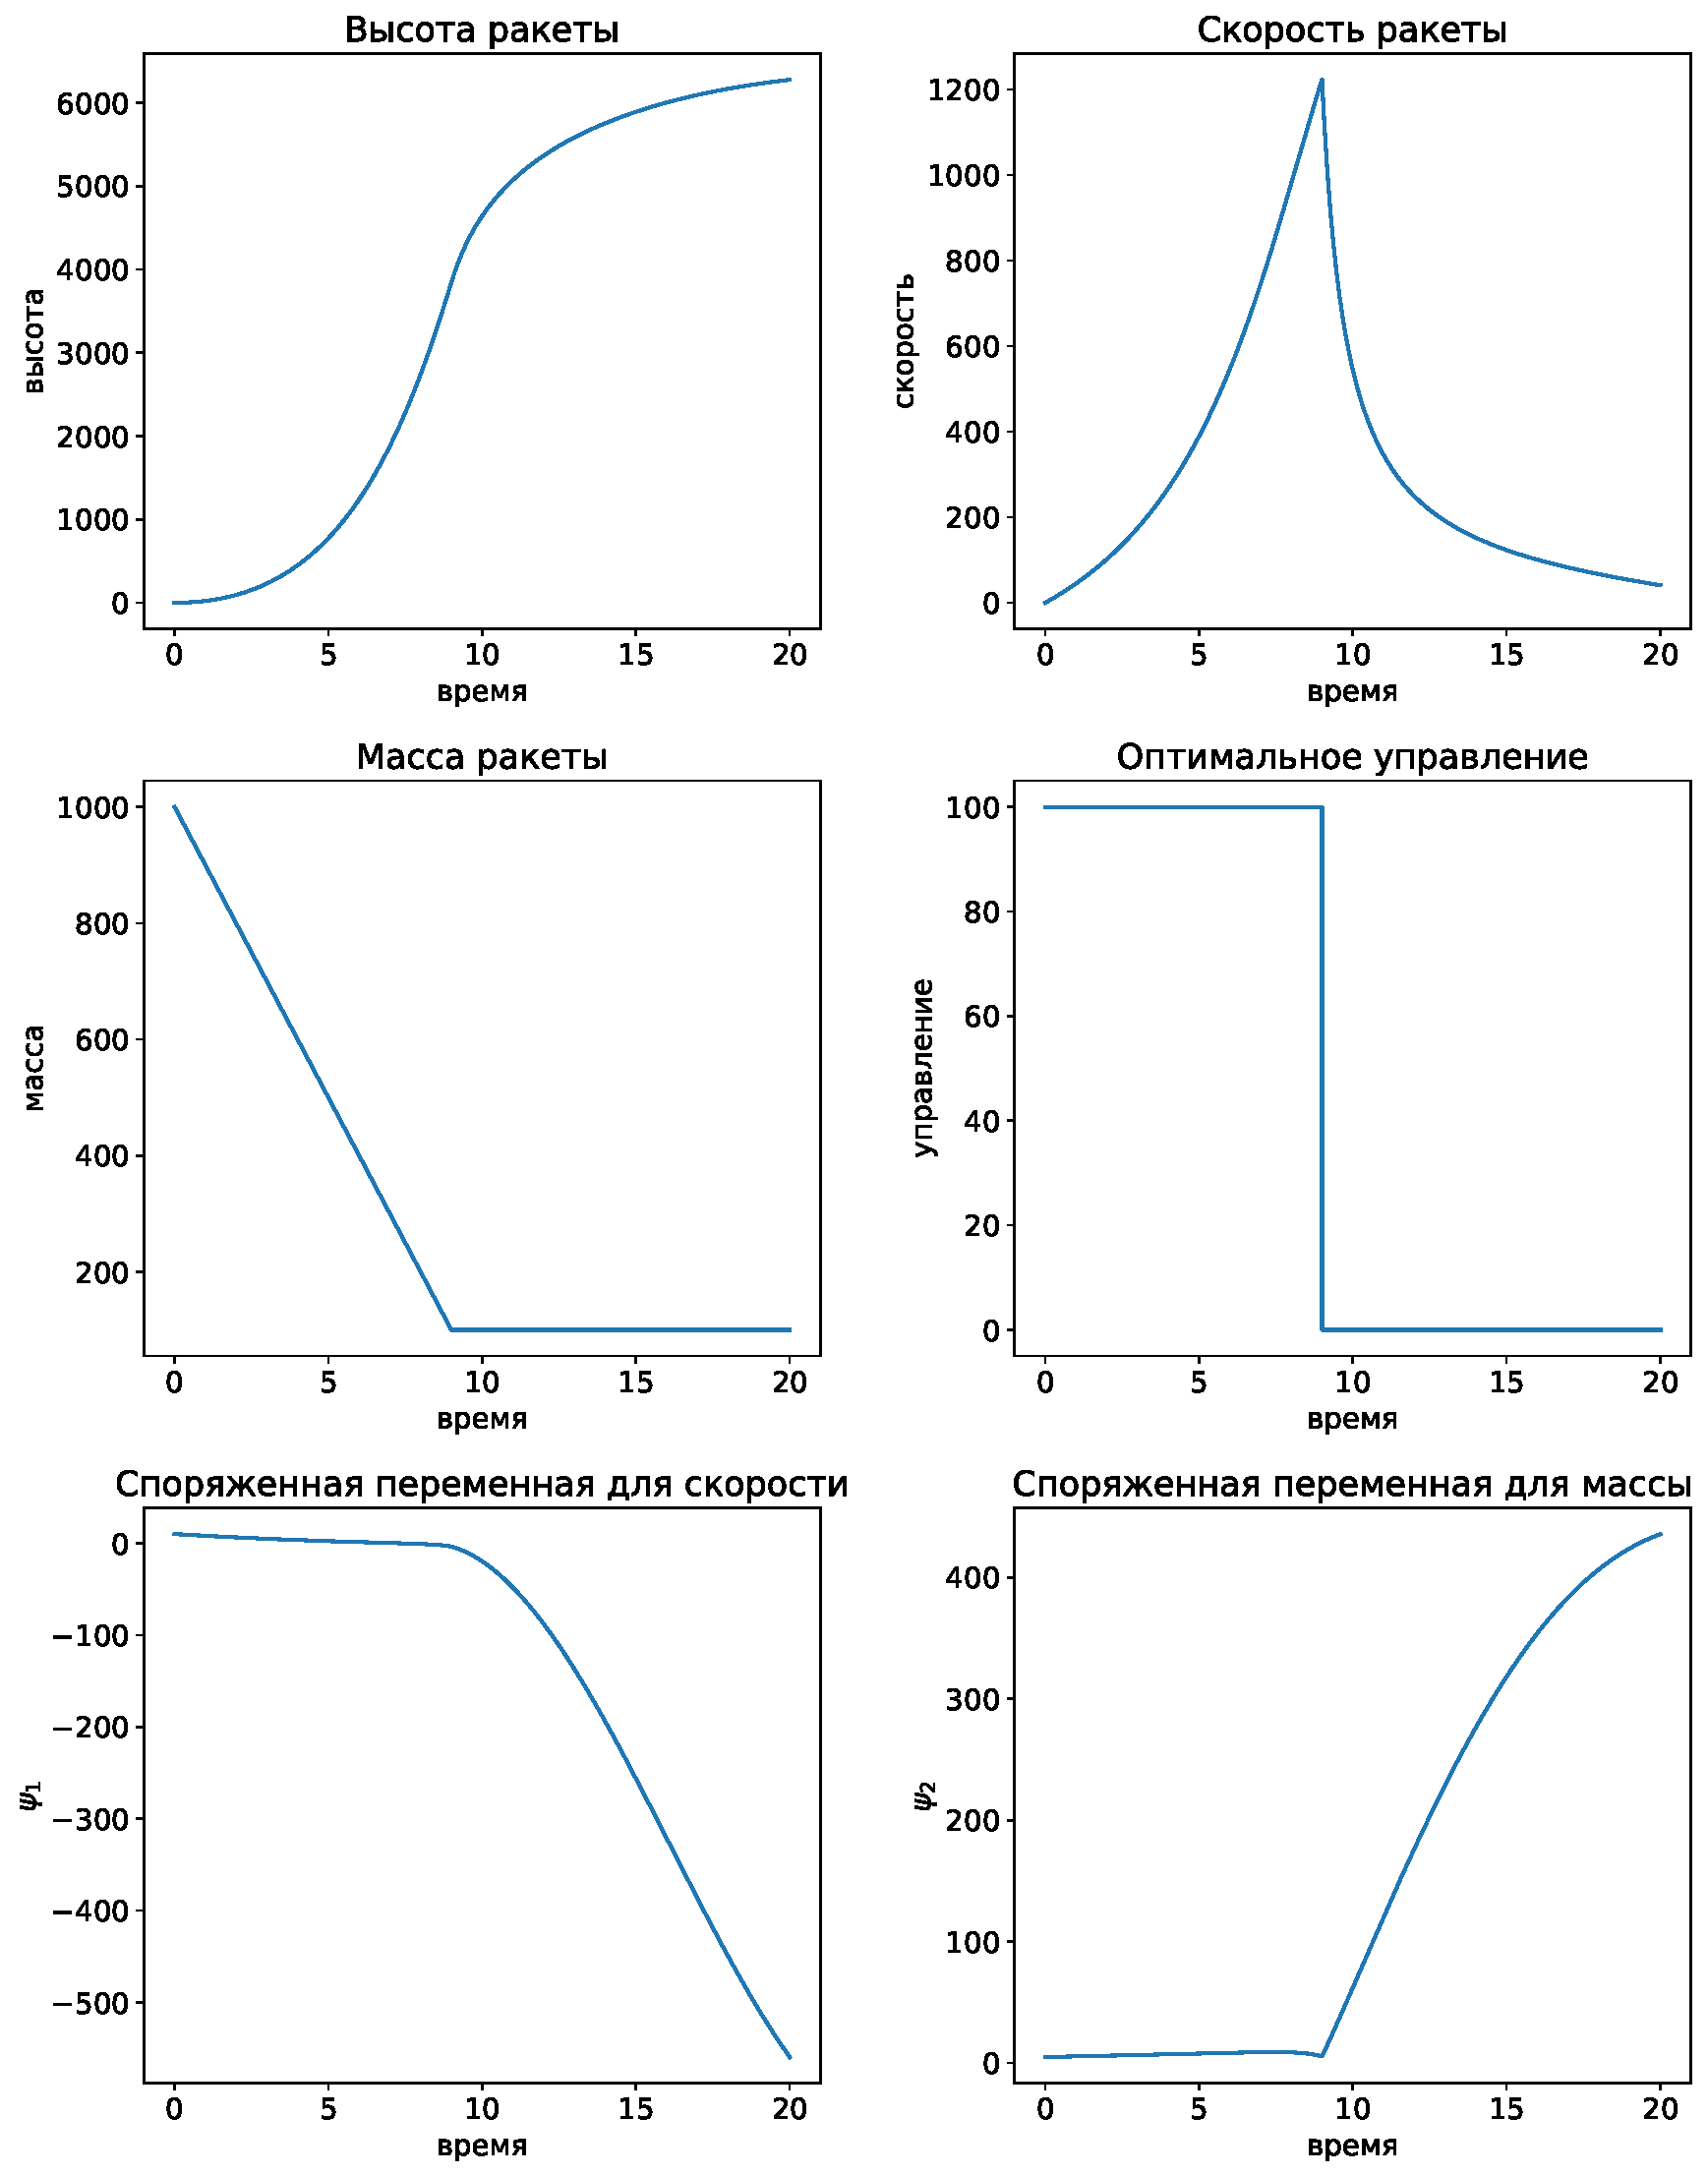
\includegraphics[width=0.9\textwidth]{1_1.pdf}
    \label{fig:1_1}
    \caption{Параметры: $m_0=1000$, $M=100$,  $l=500$,  $u_{max}=100$
        $g=10$,  $k=0.1$,  $T=20$.
        Видно, что нарушены условия трансверсальности.
        Высота $6275$.}
\end{center} 
\end{figure} 

\begin{figure}[H]
\begin{center}
    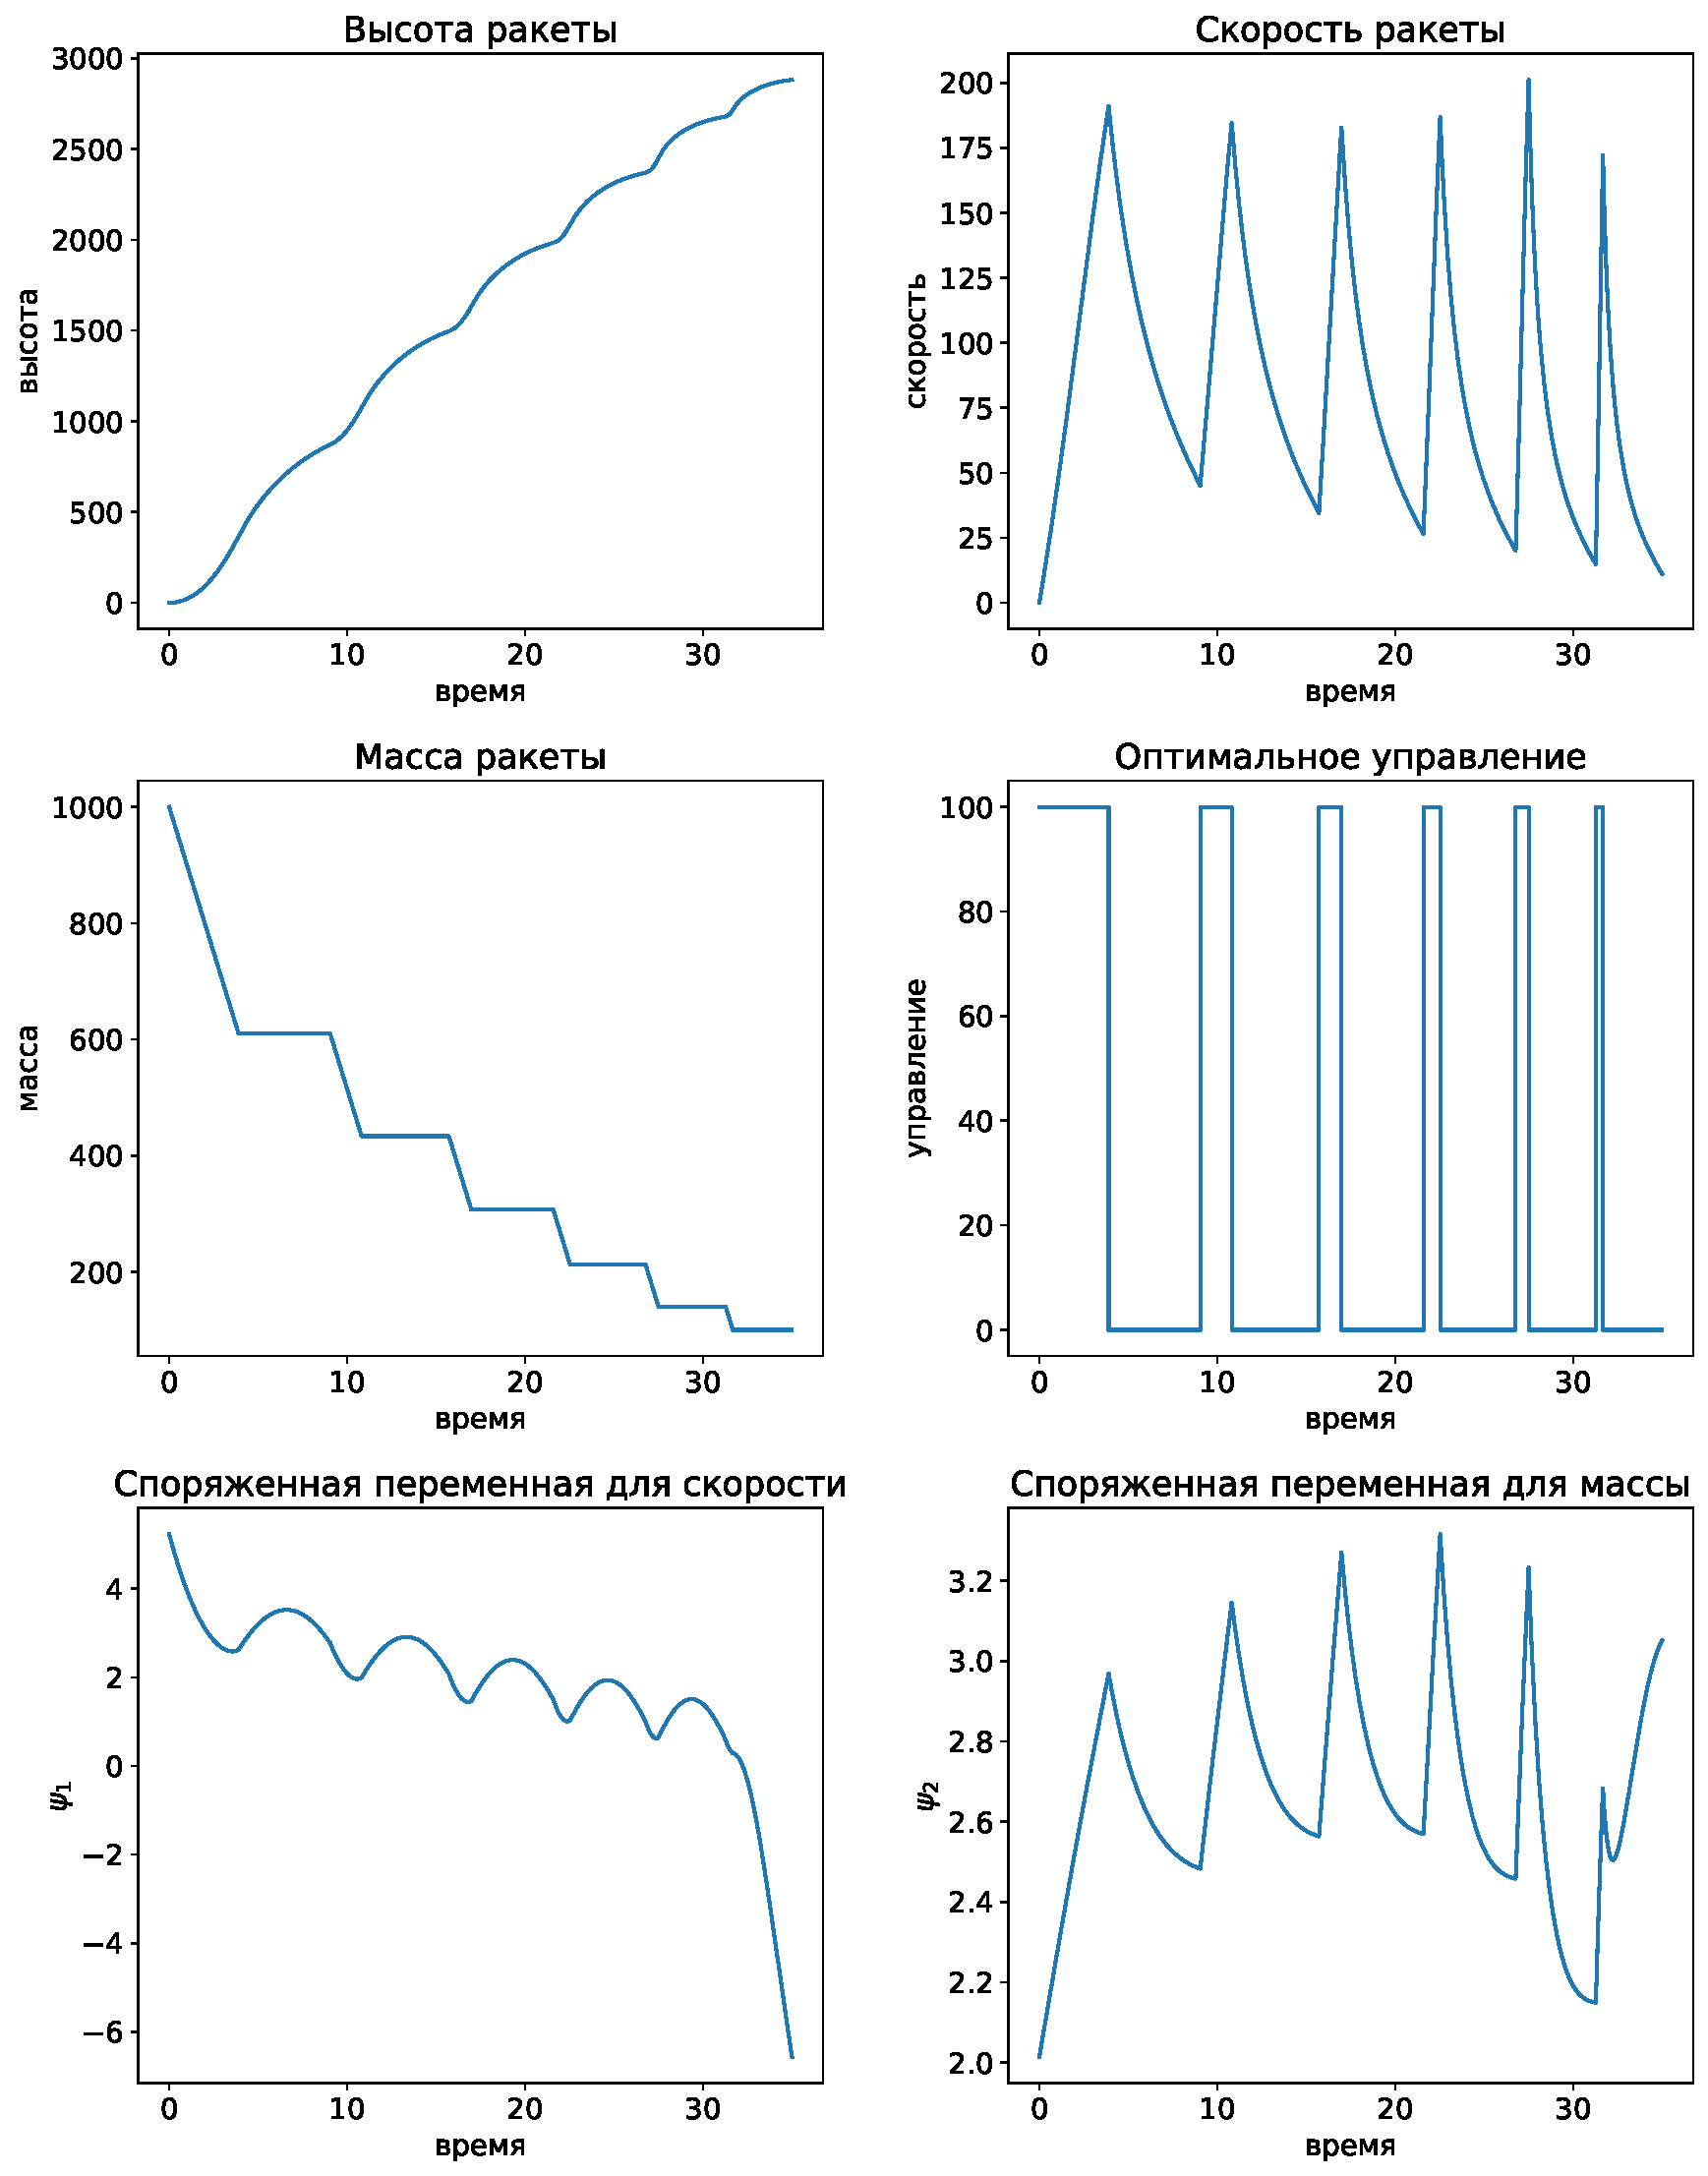
\includegraphics[width=0.9\textwidth]{1_2.pdf}
    \label{fig:1_2}
    \caption{Параметры: $m_0=1000$, $M=100$,  $l=500$,  $u_{max}=100$
        $g=10$,  $k=1$,  $T=35$.
        Высота $2881$.
        Здесь также нарушено условие трансверсальности для сопряженной переменной по скорости.
        Заметим, что если бы $T$ было, чуть меньше, то условие трансверсальности бы выполнилось ($\psi_1 = 0$).
        Но так как топливо заканчивается и мы не можем сделать еще одно переключение, то вся красота ломается.
        Поэтому непереборный алгоритм тут не работает.
        Так же в этом случае не рассматривался особый режим, из-за чего возникает большое количество переключений, которые можно избежать.}
\end{center} 
\end{figure}

\begin{figure}[H]
\begin{center}
    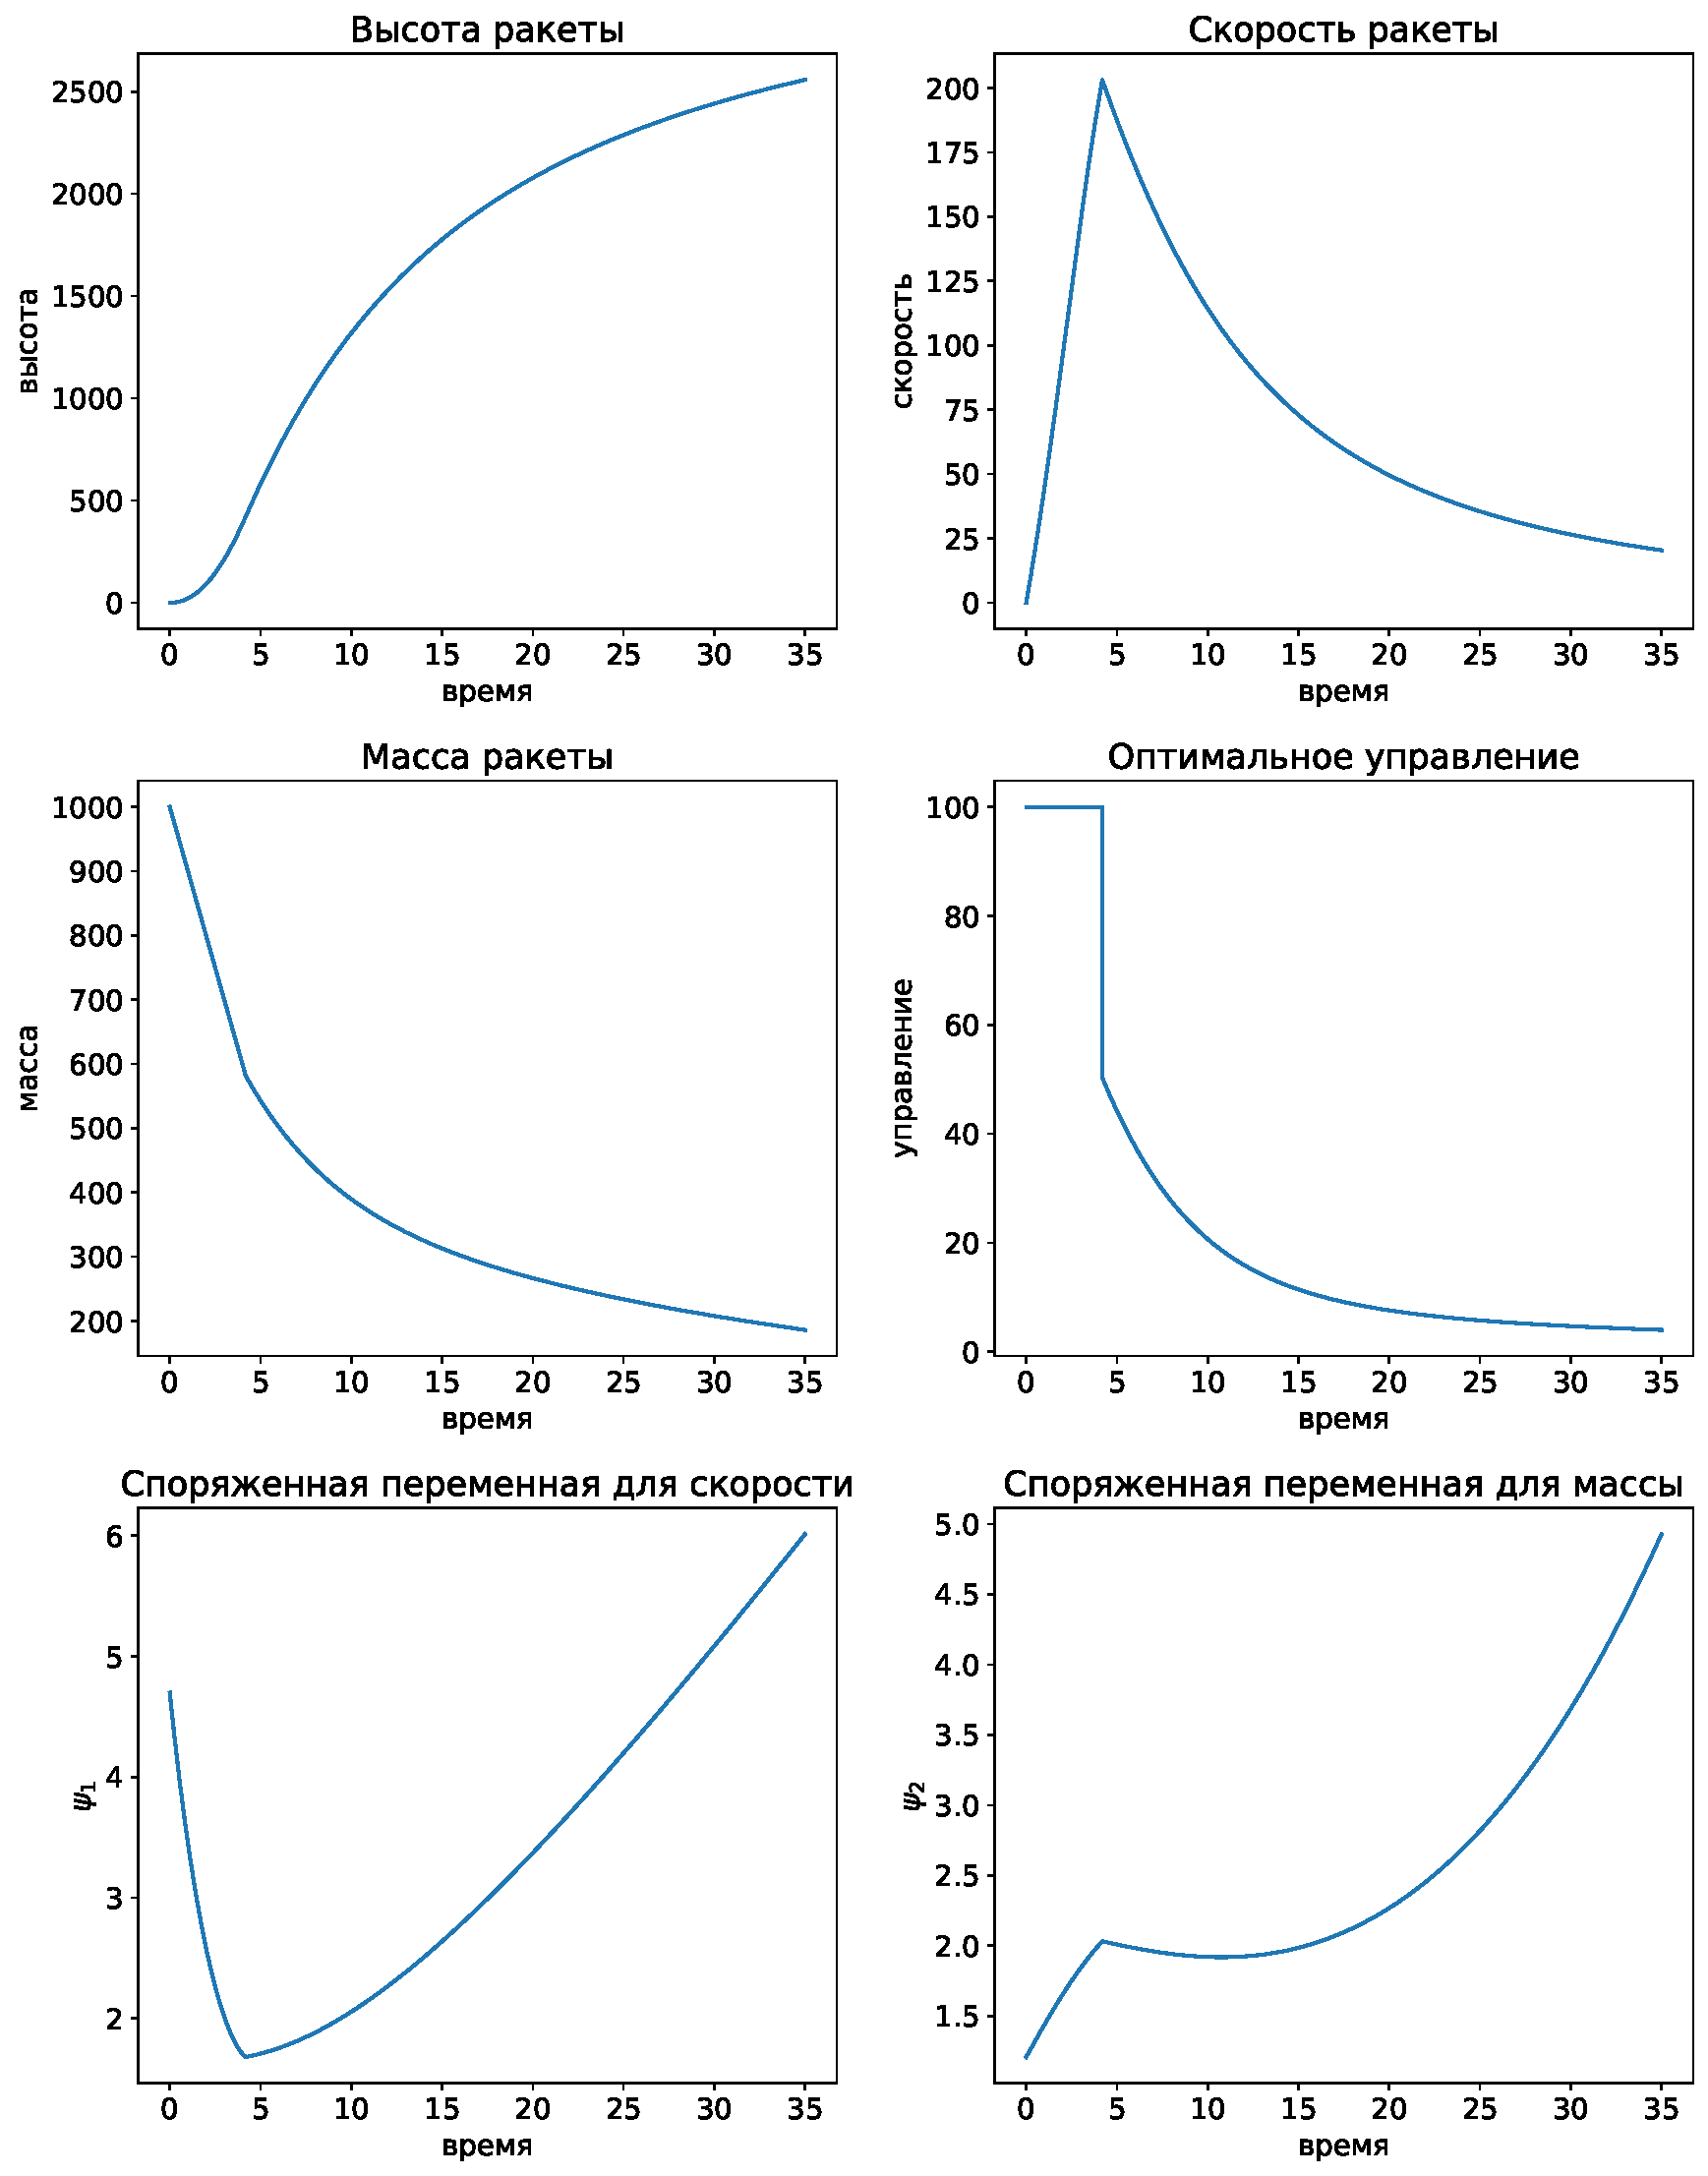
\includegraphics[width=0.9\textwidth]{1_3.pdf}
    \label{fig:1_3}
    \caption{Параметры: $m_0=1000$, $M=100$,  $l=500$,  $u_{max}=100$
        $g=10$,  $k=1$,  $T=35$.
        Высота $2558$.
        Здесь параметры такие же, как и в предыдущем слуае, но рассмотрен вариант, когда на первом переключении ракета входит в особый режим.
        Как видно, ОР не является оптимальным при данных параметрах.}
\end{center} 
\end{figure}

\begin{figure}[H]
\begin{center}
    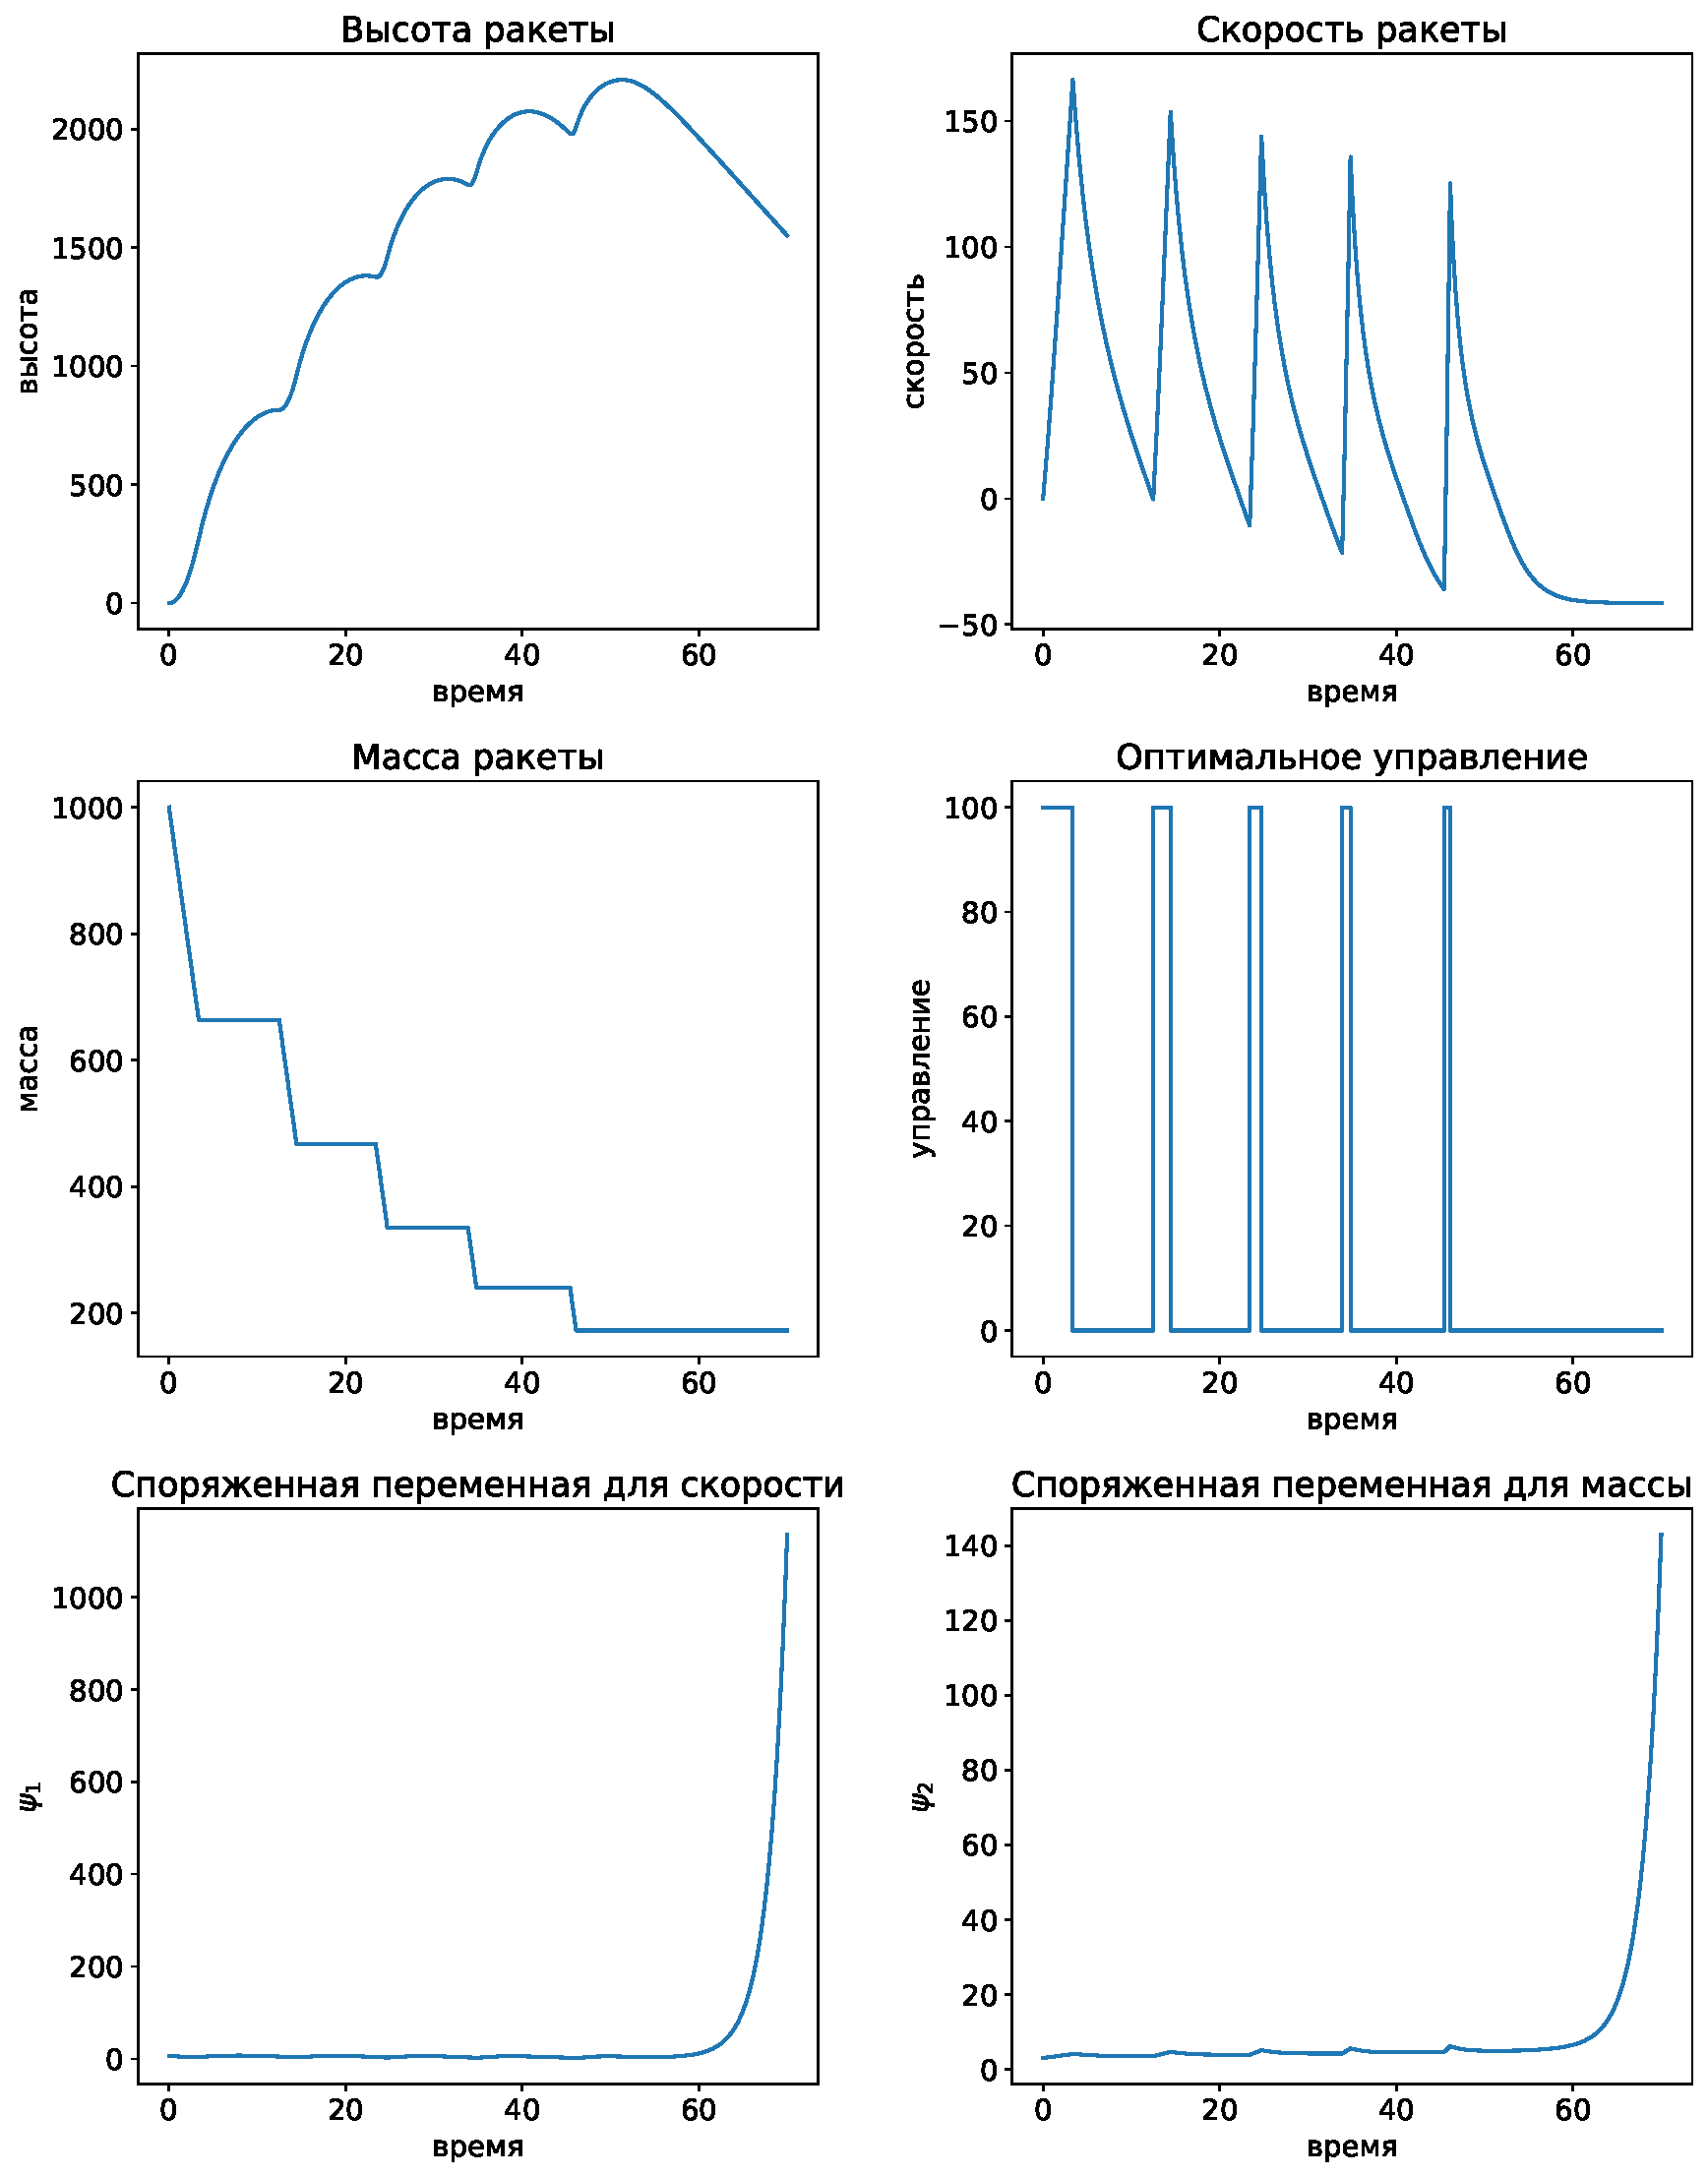
\includegraphics[width=0.9\textwidth]{1_4.pdf}
    \label{fig:1_4}
    \caption{Параметры: $m_0=1000$, $M=100$,  $l=500$,  $u_{max}=100$
        $g=10$,  $k=1$,  $T=70$.
        Высота $1550$.
        В данном случае мы увеличили временной интервал с $35$ до  $70$.
        Рассматриваются только регулярные решения.}
\end{center} 
\end{figure}

\begin{figure}[H]
\begin{center}
    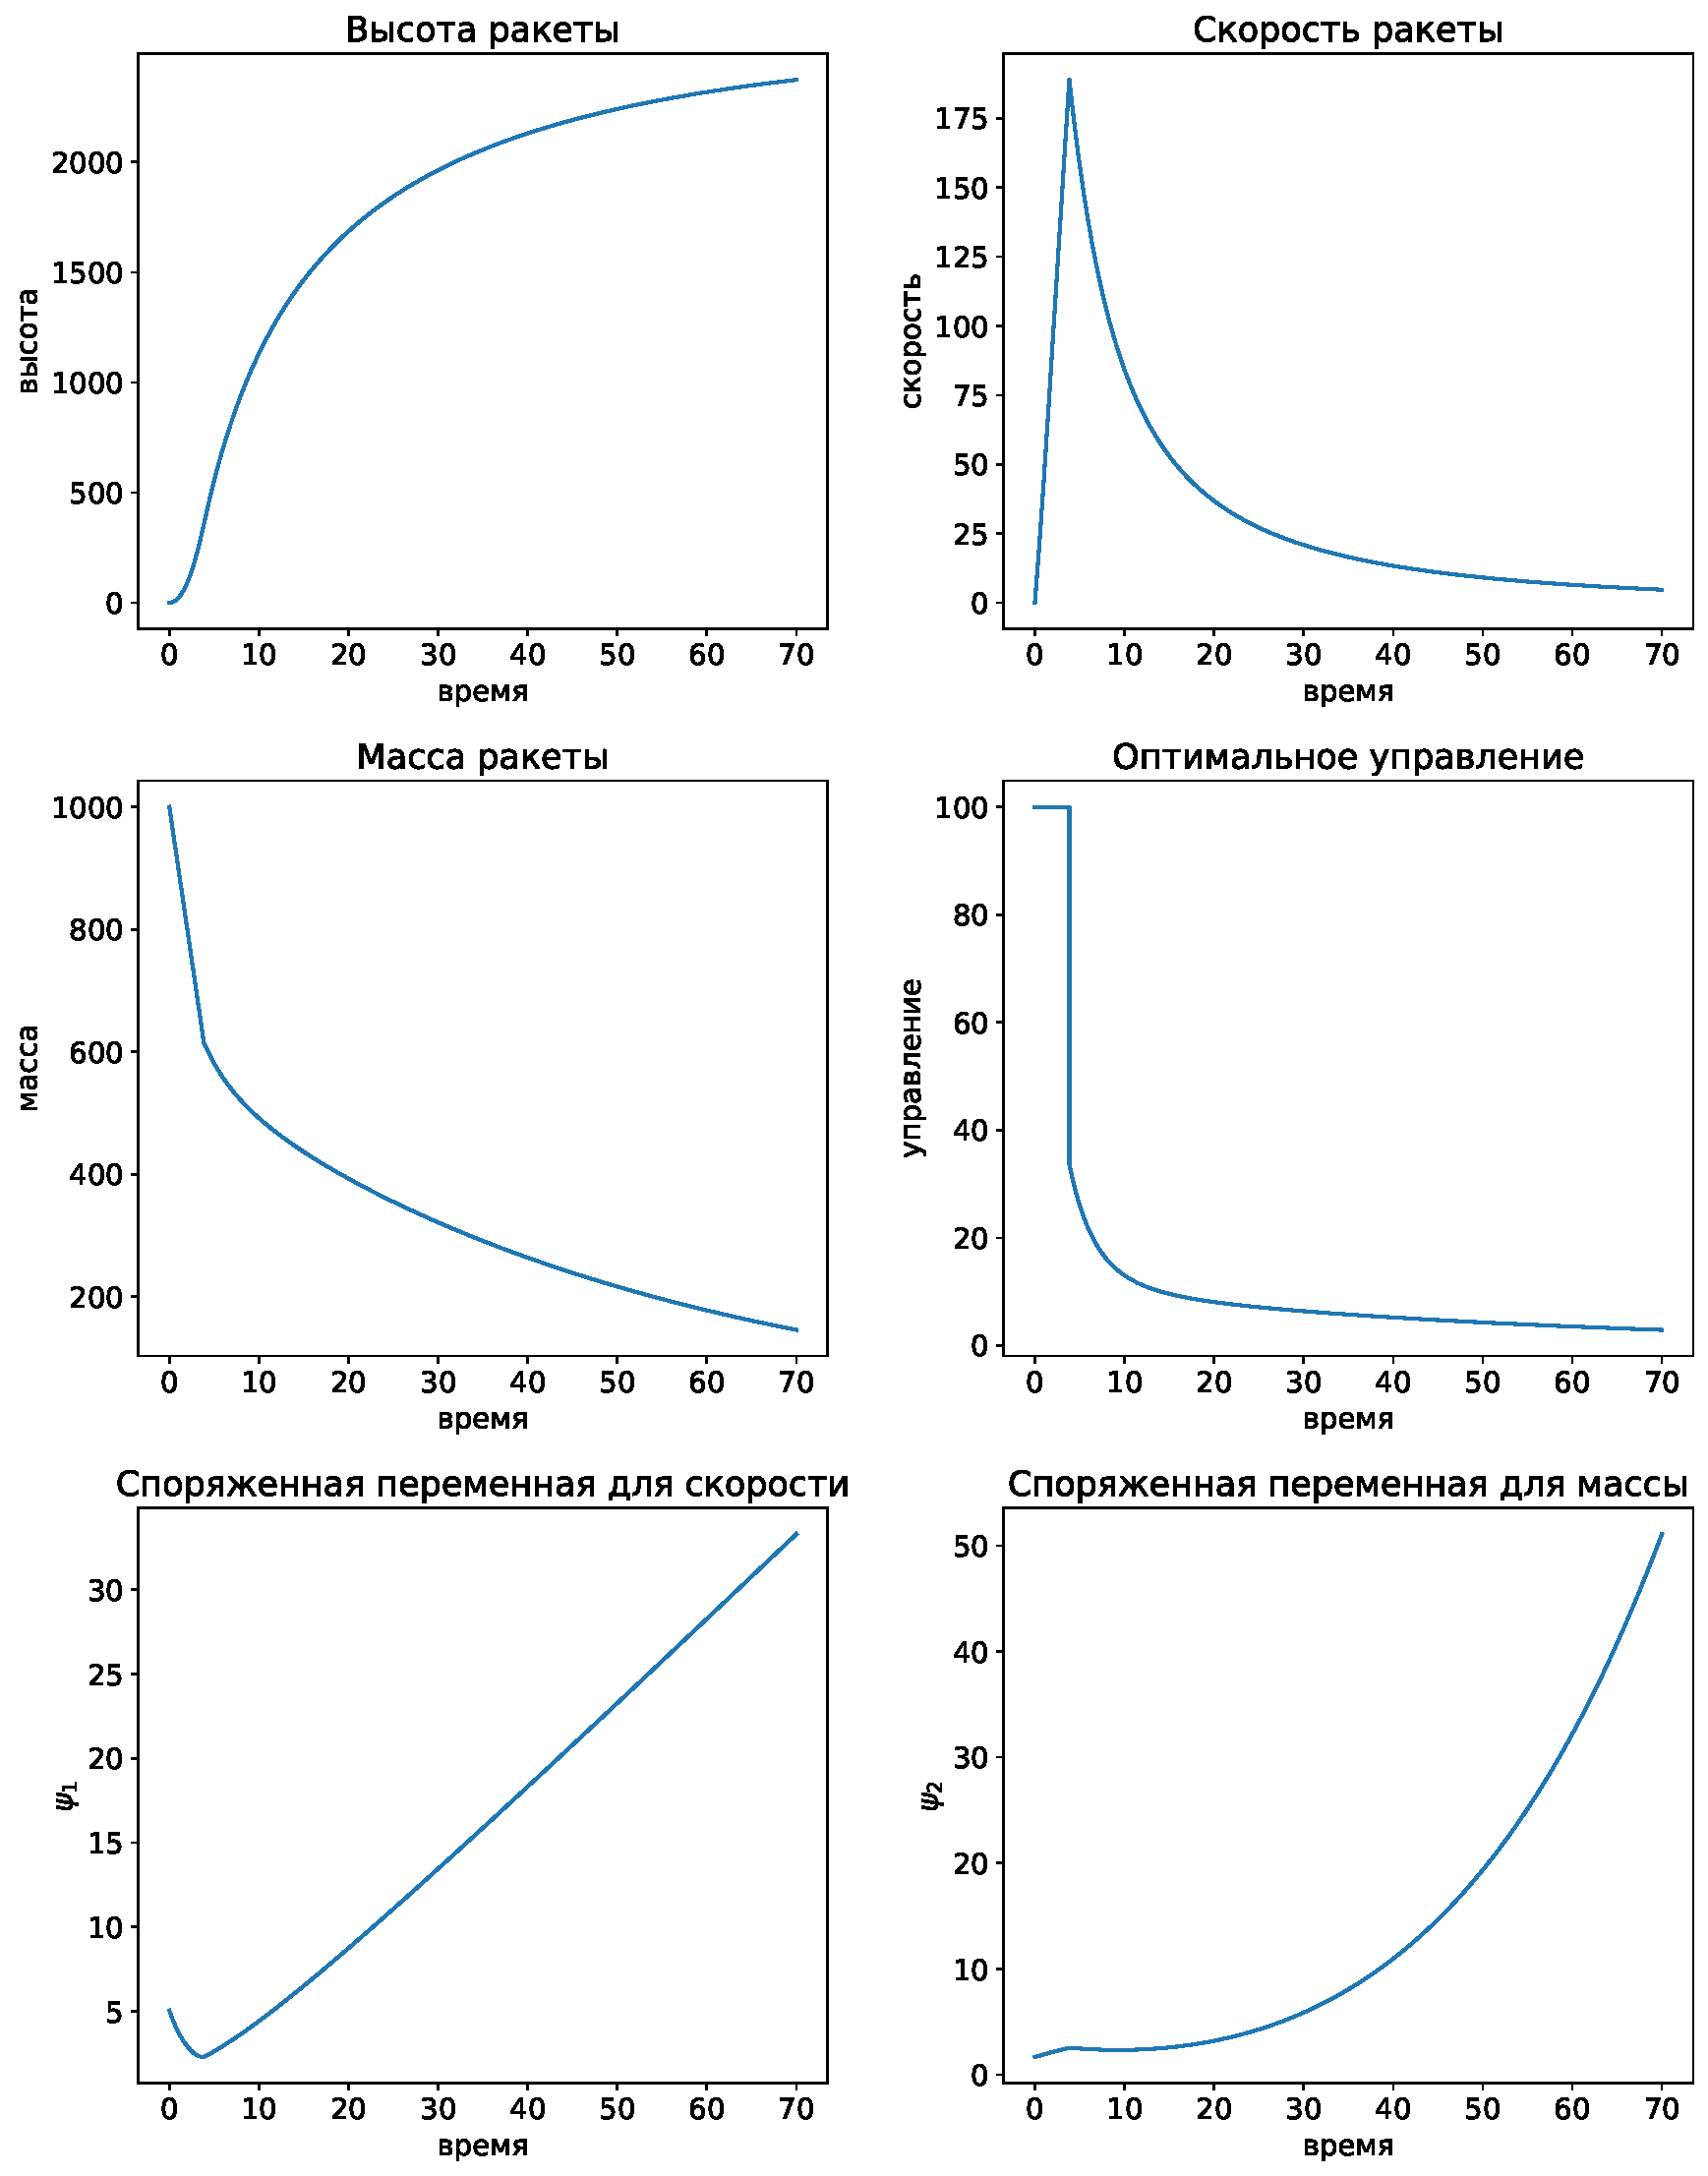
\includegraphics[width=0.9\textwidth]{1_5.pdf}
    \label{fig:1_5}
    \caption{Параметры: $m_0=1000$, $M=100$,  $l=500$,  $u_{max}=100$
        $g=10$,  $k=1$,  $T=70$.
        Высота $2373$.
        Однако если при данных параметрах рассмотреть особый режим, то виден выйгрыш в высоте примерно в 1,5 раза.}
\end{center} 
\end{figure}

\section{Решение задачи 2}

Как и в предыдущей задаче, положим $x_1 = v$, и $x_2 = m$. 
Дополнительно введем переменную $x_3$, отвечающую за высоту.
Тогда система приобретает следующий вид:

\begin{equation}
    \begin{cases}
        \displaystyle
        \dot x_1 = -g - \frac{kx_1^2}{x_2} + \frac{u}{x_2}(l + x_1) \\
        \displaystyle
        \dot x_2 = -u \\
        \displaystyle
        \dot x_3 = x_1 \\
        \displaystyle
        \int\limits_{0}^{T} e^{-\alpha t} u(t)\,dt \rightarrow \min.
    \end{cases} 
\end{equation} 
Функция Гамильтона-Понтрягина:
\begin{equation}
    \mathscr{H} = \psi_0 e^{-\alpha t} u(t) +
    \psi_1 \left[ -g - \frac{kx_1^2}{x_2} + \frac{u}{x_2}(l + x_1) \right] -
    \psi_2 u + \psi_3 x_3
.\end{equation}
Сопряженная система:
\begin{equation}\label{eq:1_conj}
\begin{cases}
    \displaystyle
    \dot \psi_1 = -\psi_0 + \frac{2k\psi_1x_1^2}{x_2} -
        \frac{\psi_1 u}{x_2} \\
    \displaystyle
    \dot \psi_2 = -\frac{k\psi_1x_1^2}{x_2^2} +
        \frac{\psi_1u}{x_2^2}(l + x_1) \\
    \dot \psi_3 = 0.
\end{cases}     
\end{equation}
Заданы следующие ограничения на значения переменный в начале и в конце:
\[
    x_1(0) = 0, \quad x_2(0) = 0, \quad x_3(0) = 0, \quad 
    u(0) \ge \frac{m_0 g}{l}
.\]
Последнее из этих условий гарантирует, что ракета не упадет в начале.
Также заданы условия на правом конце и условия трансверсальности:
\[
    \psi_1(T) = 0,\quad x_3(T) = H
.\] 
Как и в предыдущей задаче определим функцию, от значений которой будет зависеть управление:
\begin{equation}\label{eq:2_F}
    F = \psi_0 x_2 e^{-\alpha t} + \psi_1(x_1 + l) - \psi_2 x_2
.\end{equation} 
Тогда оптимальное управление:
\begin{equation}\label{eq:1_opt_control}
    u^* = \left\{
    \begin{aligned}
        u_{max}, \quad &\text{если}\ F > 0, \\
        [0, u_{max}], \quad &\text{если}\ F = 0, \\
        0, \quad &\text{если}\ F < 0,
    \end{aligned} 
    \right.
\end{equation} 

\subsection{Анормальный случай}
В данной задаче анормальный случай является просто задачей 1, 
поэтому считаем, что анормальный случай уже рассмотрен и далее будет 
рассматриватсья только случай, когда $\psi_0 \equiv -1$.

\subsection{Особый режим}
Рассмеотрение особого режима практически не отличается от 1 задачи:
точно так же рассматриваются первая и вторая производная функции~\eqref{eq:2_F}.
Различия в управлении в особом режиме минимальны: по одному слагаемому добавляется в числитель и знаменатель дроби:
\begin{equation}
    u^*_{sm} =  \frac{\alpha^2 x_2^3 e^{-\alpha t} + 2 g k l \psi_{1} x_{2} + 6 g k \psi_{1} x_{1} x_{2} - 2 g x_{2}^{2} - 2 k^{2} l \psi_{1} x_{1}^{2} + 2 k l x_{1} x_{2} + k x_{1}^{2} x_{2}}{-\alpha x_2^2 e^{-\alpha t} + g \psi_{1} x_{2} + 2 k l^{2} \psi_{1} + 6 k l \psi_{1} x_{1} + 4 k \psi_{1} x_{1}^{2} - l x_{2} - x_{1} x_{2}}
.\end{equation} 

\subsection{Алгоритм численного решения}

Отличия от алгоритма решения задачи 1 несущественны.
Здесь так же рассматривается переборный алгоритм по начальным условиям на сопряженные переменный.
Рассматривать $\psi_3$ нет необходимости, так как переключения между режимами не зависят от нее. 
Потому перебором по начальным условиям находятся все управления, подозрительные на оптимальные и затем среди них выбирается то, которое приводит на высоту, максимально близкую к $H$.
Так же, как и в первой задаче отдельно рассматриваются решения без ОР и с ОР.

\subsection{Результаты численного моделирования}

\begin{figure}[H]
\begin{center}
    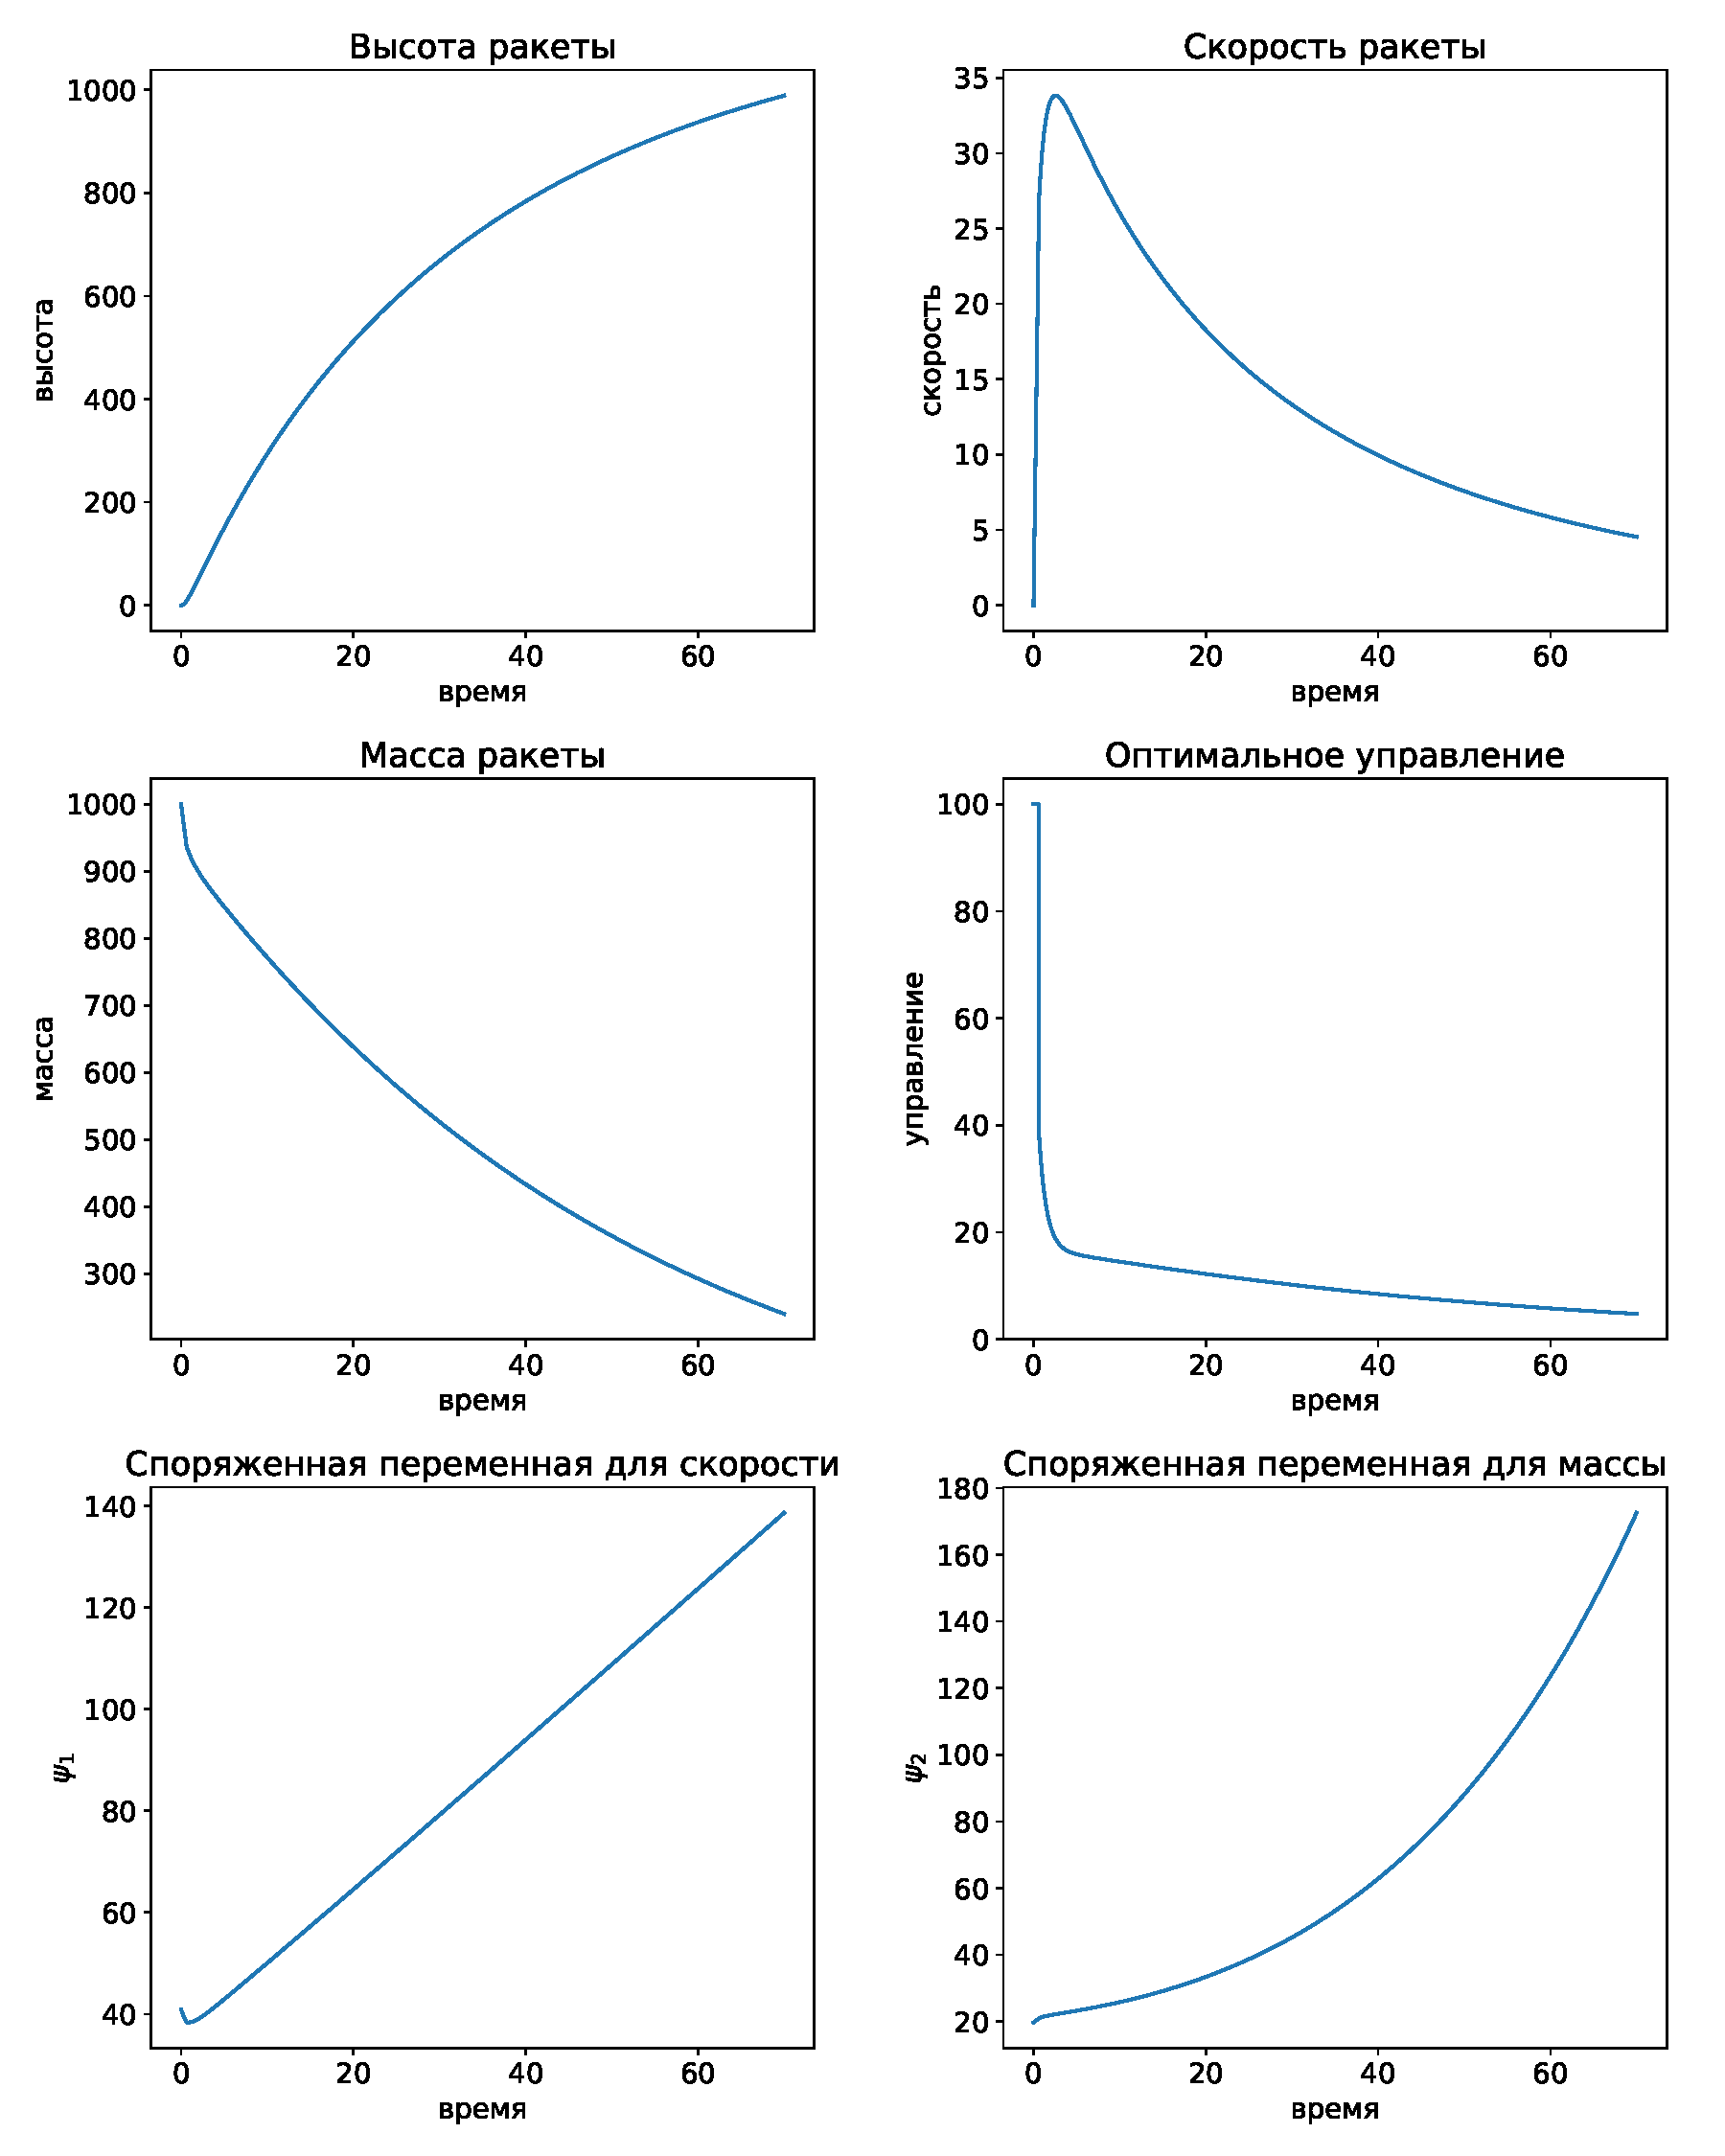
\includegraphics[width=0.9\textwidth]{2_1.pdf}
    \label{fig:1_5}
    \caption{Параметры: $m_0=1000$, $M=100$,  $l=500$,  $u_{max}=100$
        $g=10$,  $k=1$,  $T=70$, $\alpha=1$,  $H=1000$.
        Значение функционала: $3{,}0757$.
        Как видно, при данных параметрах оптимальным будет ОР.}
\end{center} 
\end{figure}

\begin{figure}[H]
\begin{center}
    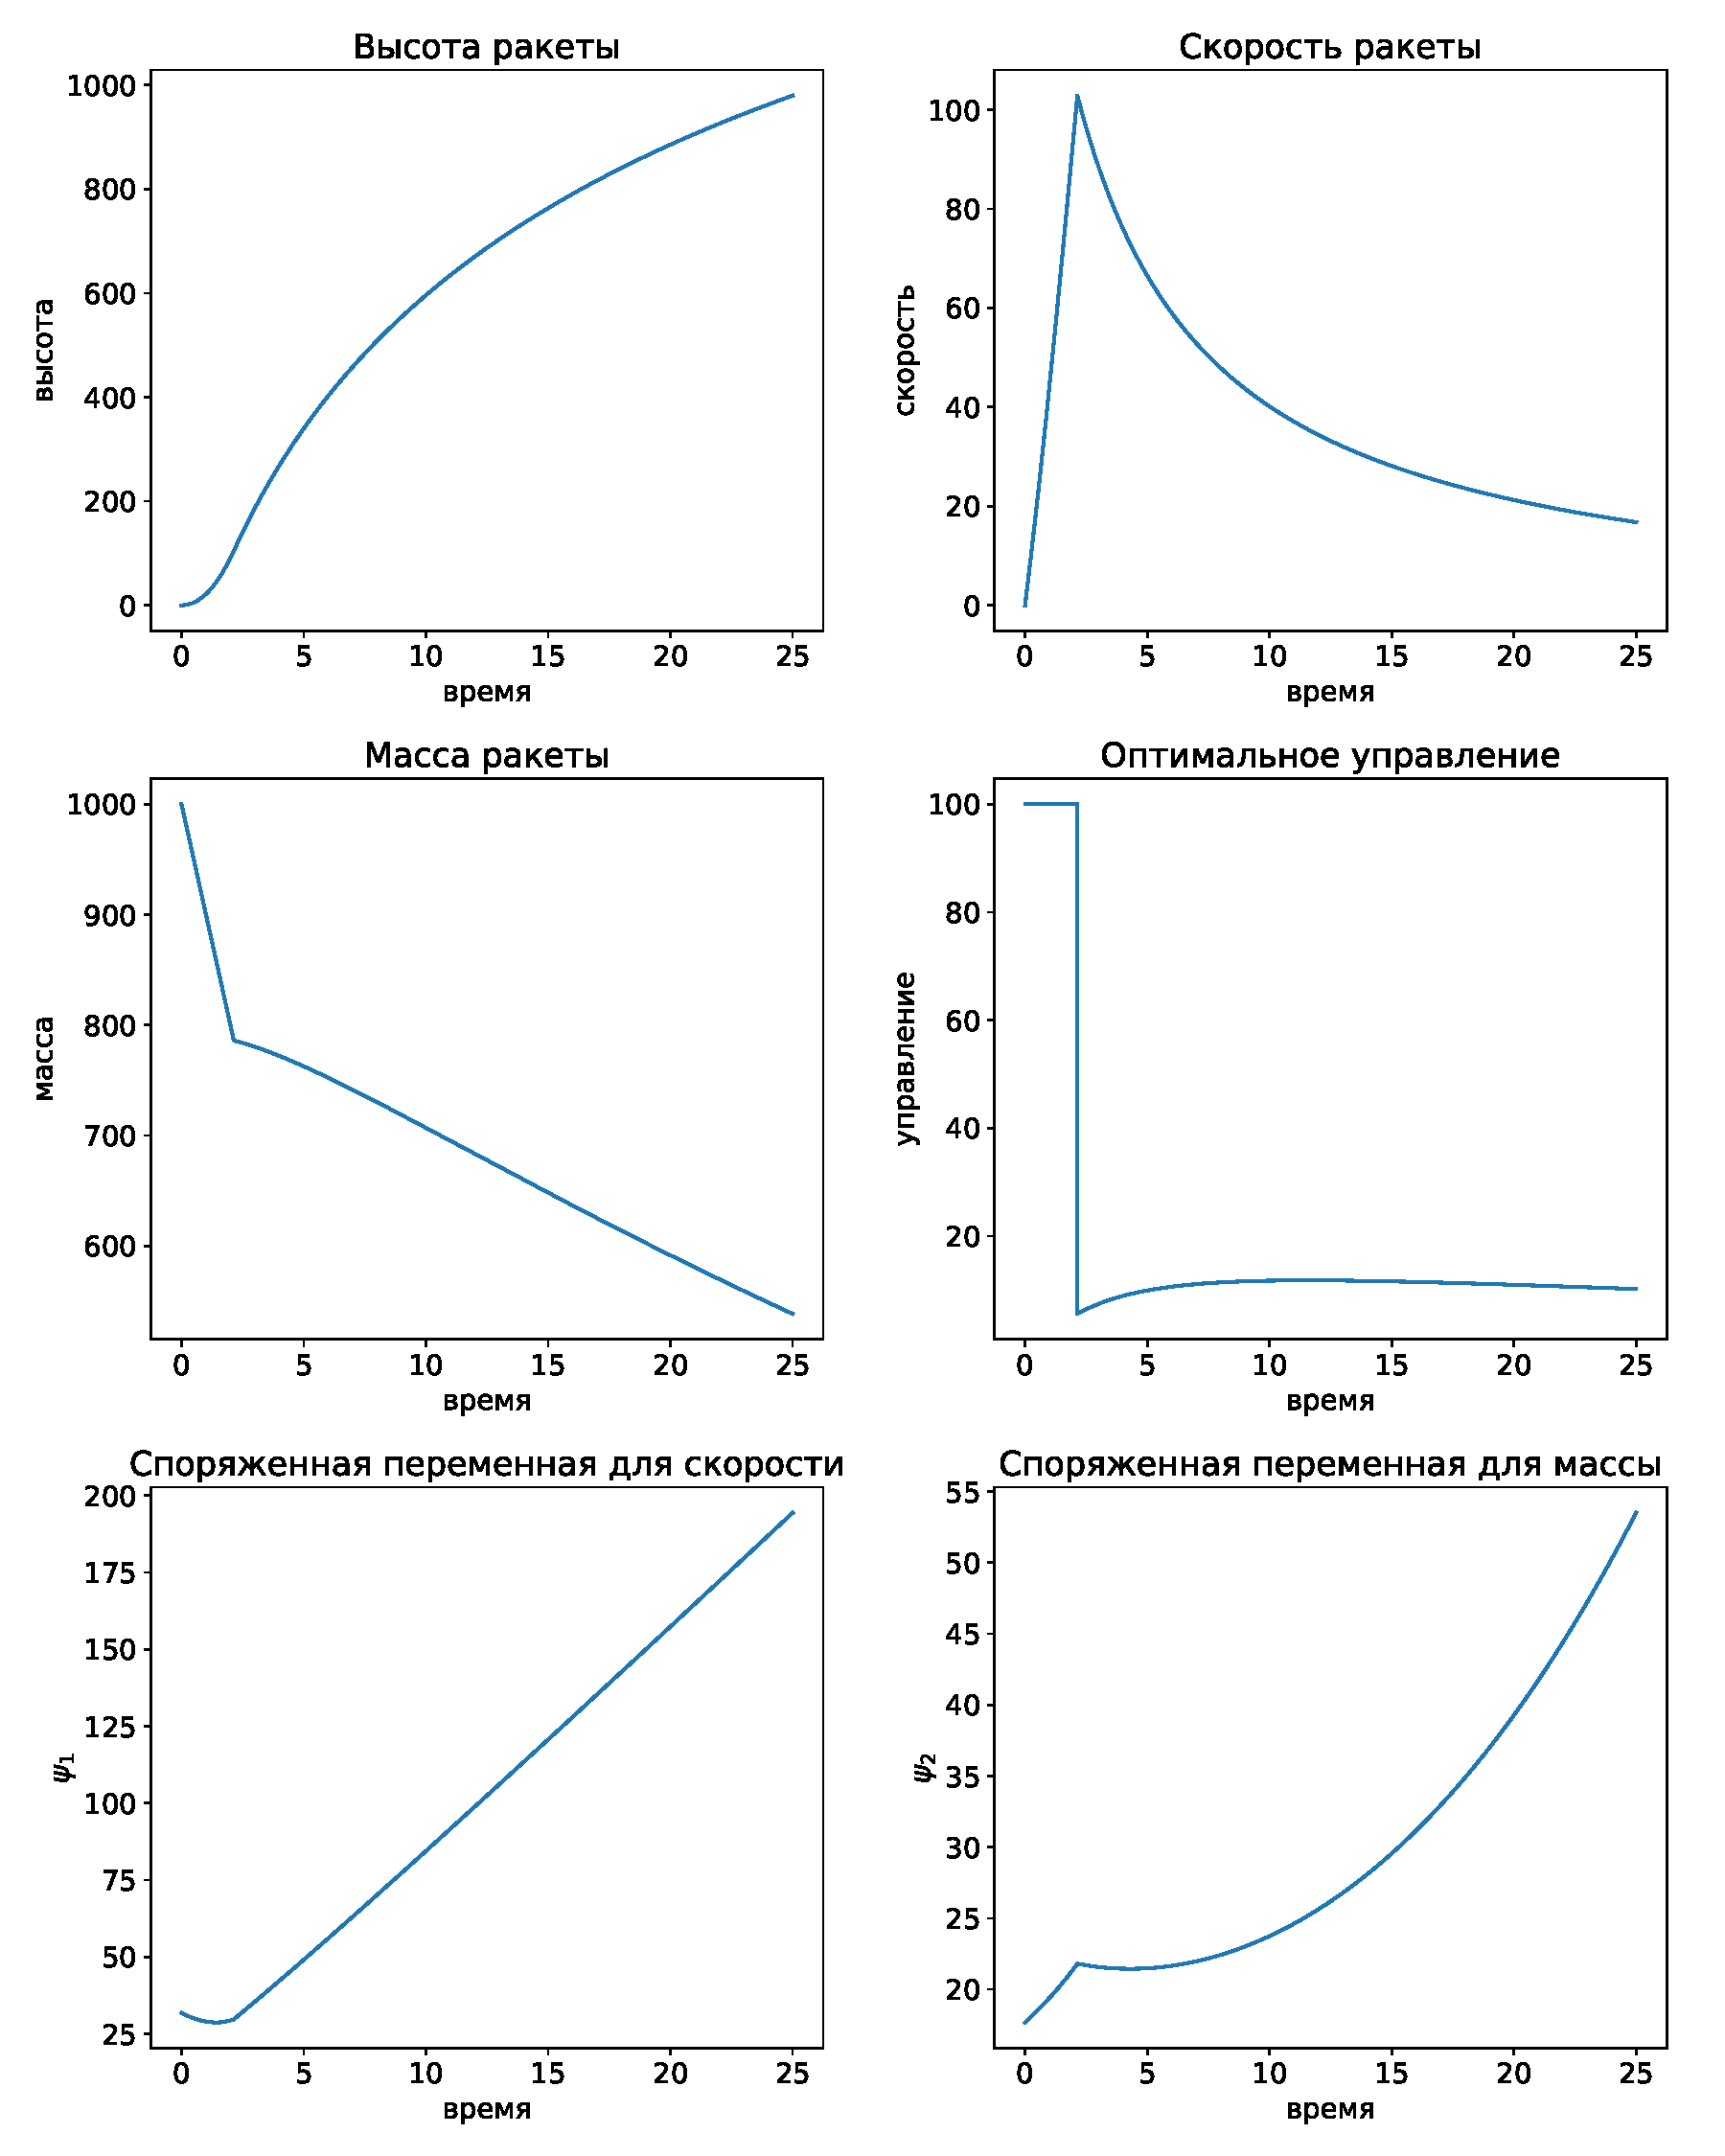
\includegraphics[width=0.9\textwidth]{2_2.pdf}
    \label{fig:1_5}
    \caption{Параметры: $m_0=1000$, $M=100$,  $l=500$,  $u_{max}=100$
        $g=10$,  $k=1$,  $T=25$, $\alpha=10^{-3}$,  $H=1000$.
        Значение функционала: $221{,}38$.
        Здесь также выгоден ОР.}
\end{center} 
\end{figure}

\begin{figure}[H]
\begin{center}
    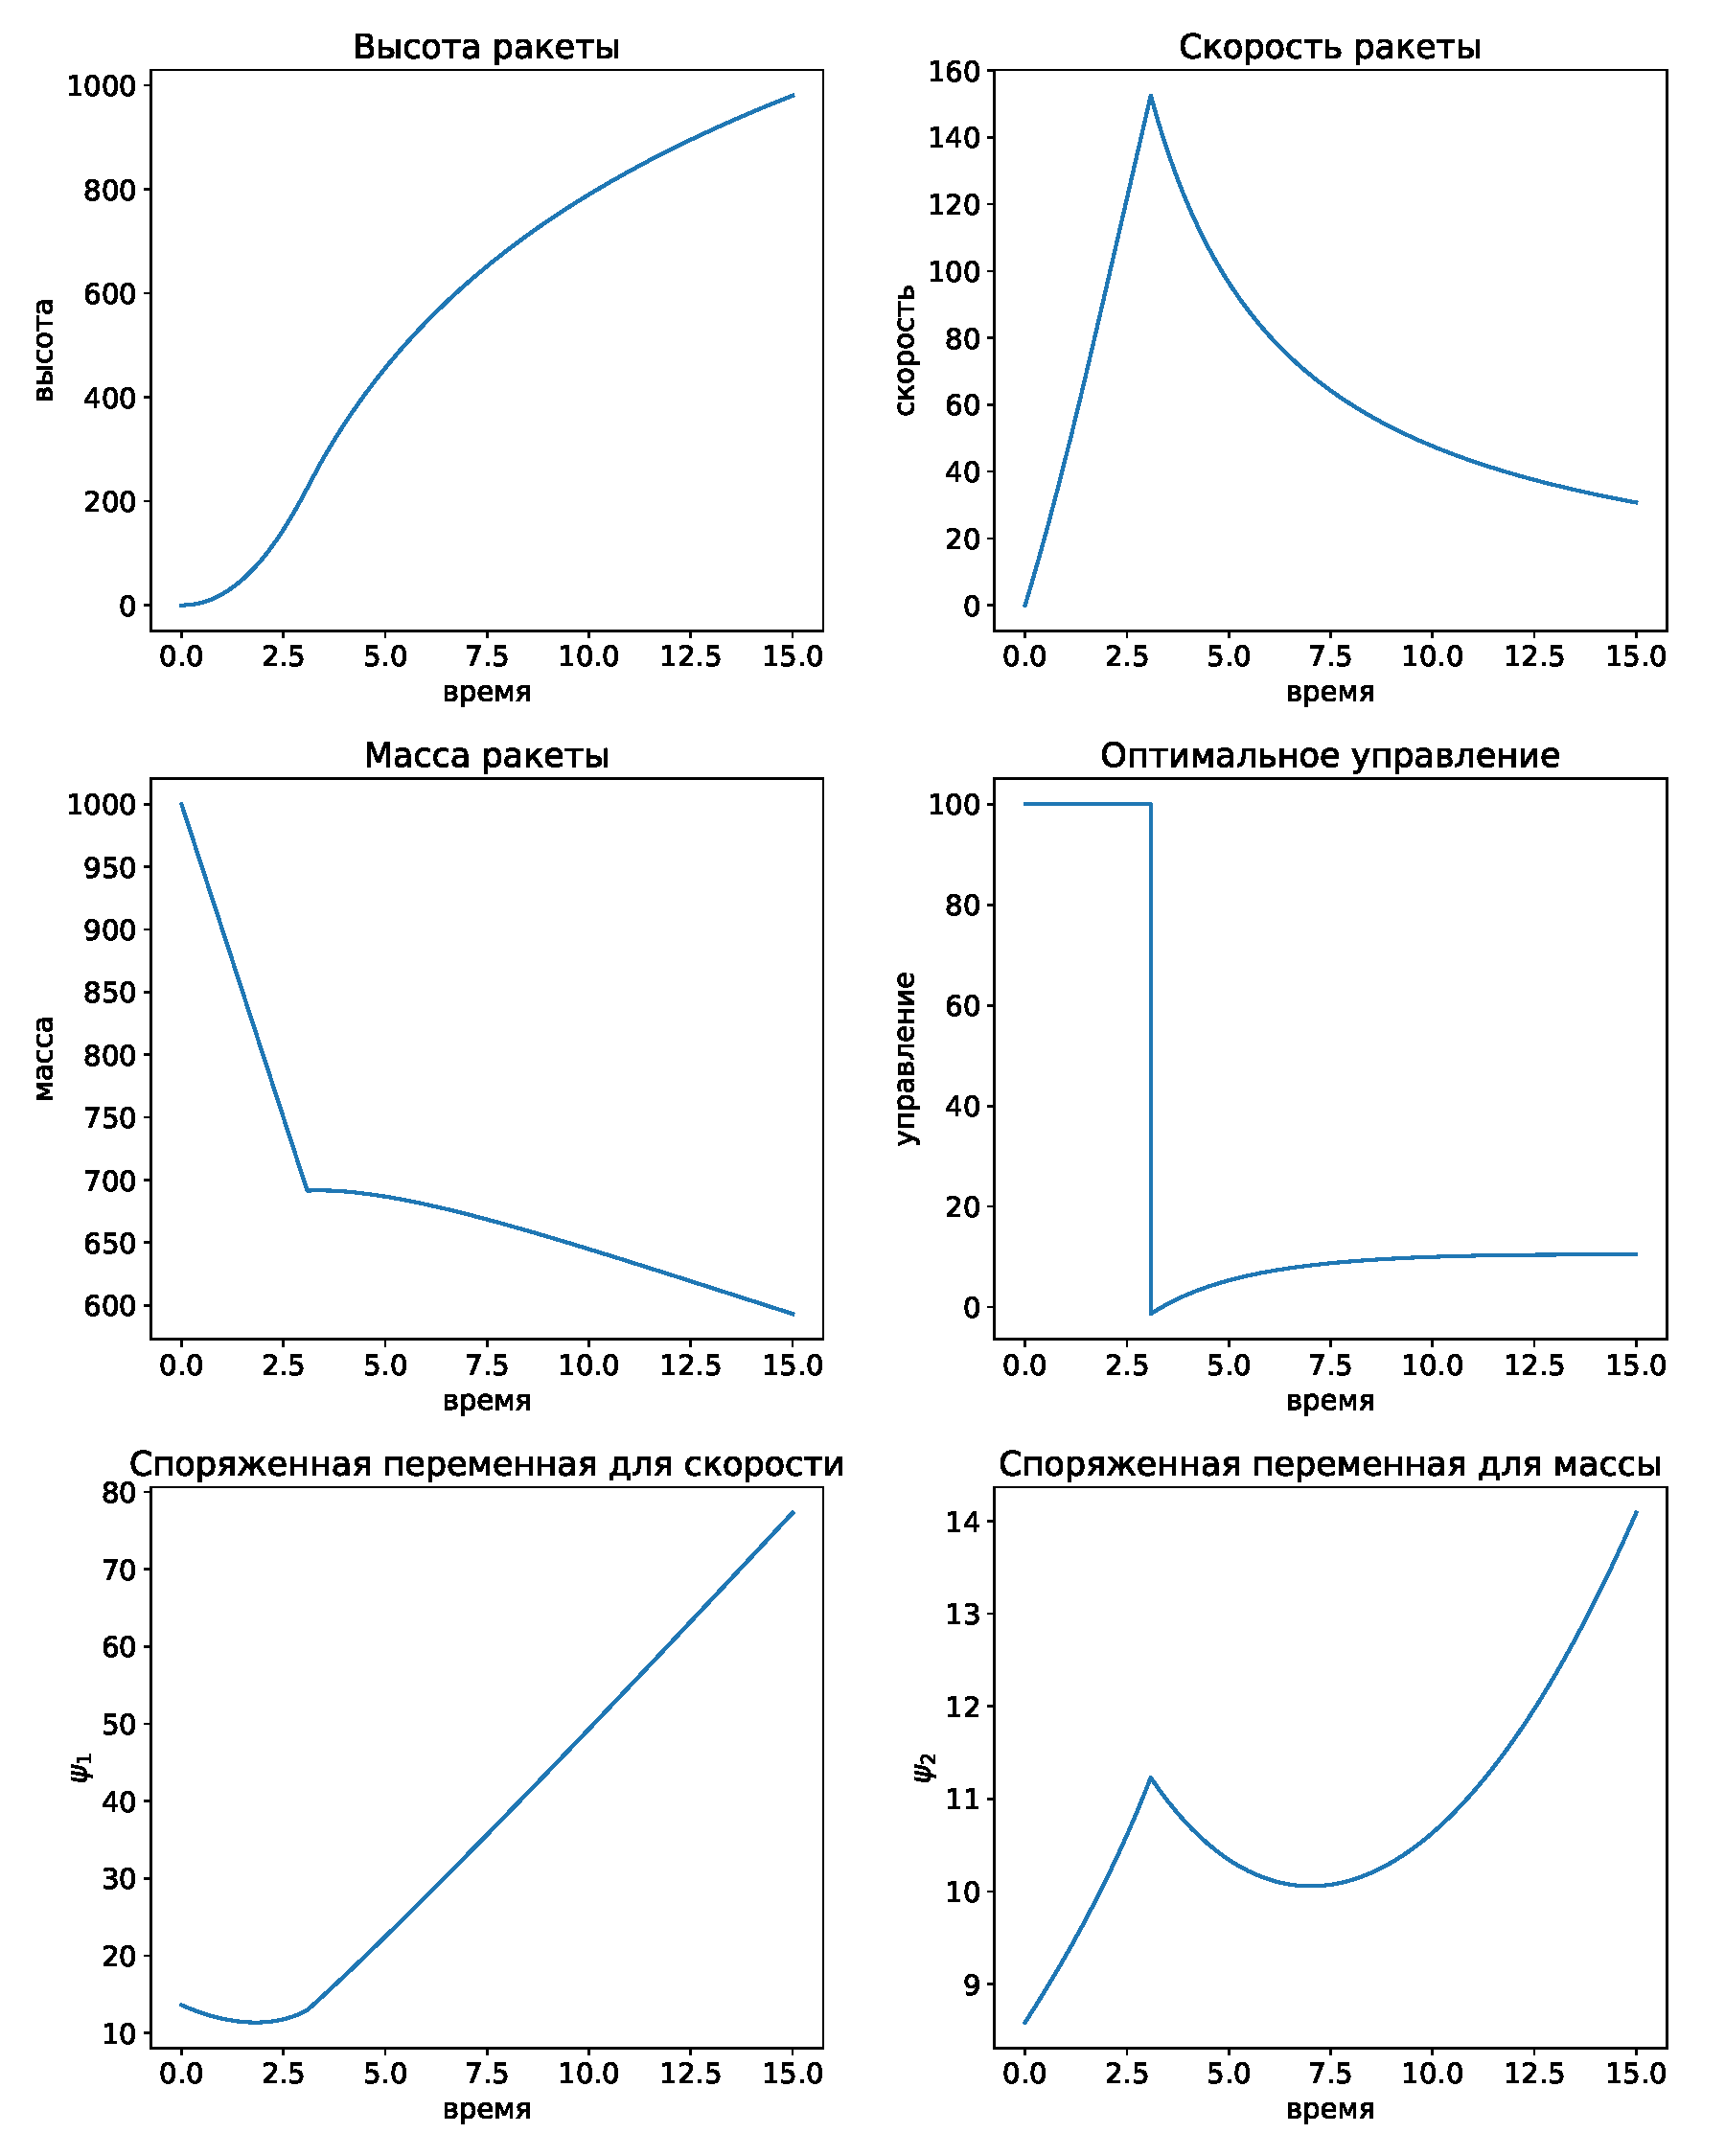
\includegraphics[width=0.9\textwidth]{2_3.pdf}
    \label{fig:1_5}
    \caption{Параметры: $m_0=1000$, $M=100$,  $l=500$,  $u_{max}=100$
        $g=10$,  $k=1$,  $T=15$, $\alpha=10^{-3}$,  $H=1000$.
        Значение функционала: $13{,}63$.
        Снова ОР.}
\end{center} 
\end{figure}

\bibliographystyle{utf8gost705u}
\bibliography{biblio}

 \end{document} 
